\begin{figure*}
    \centering
    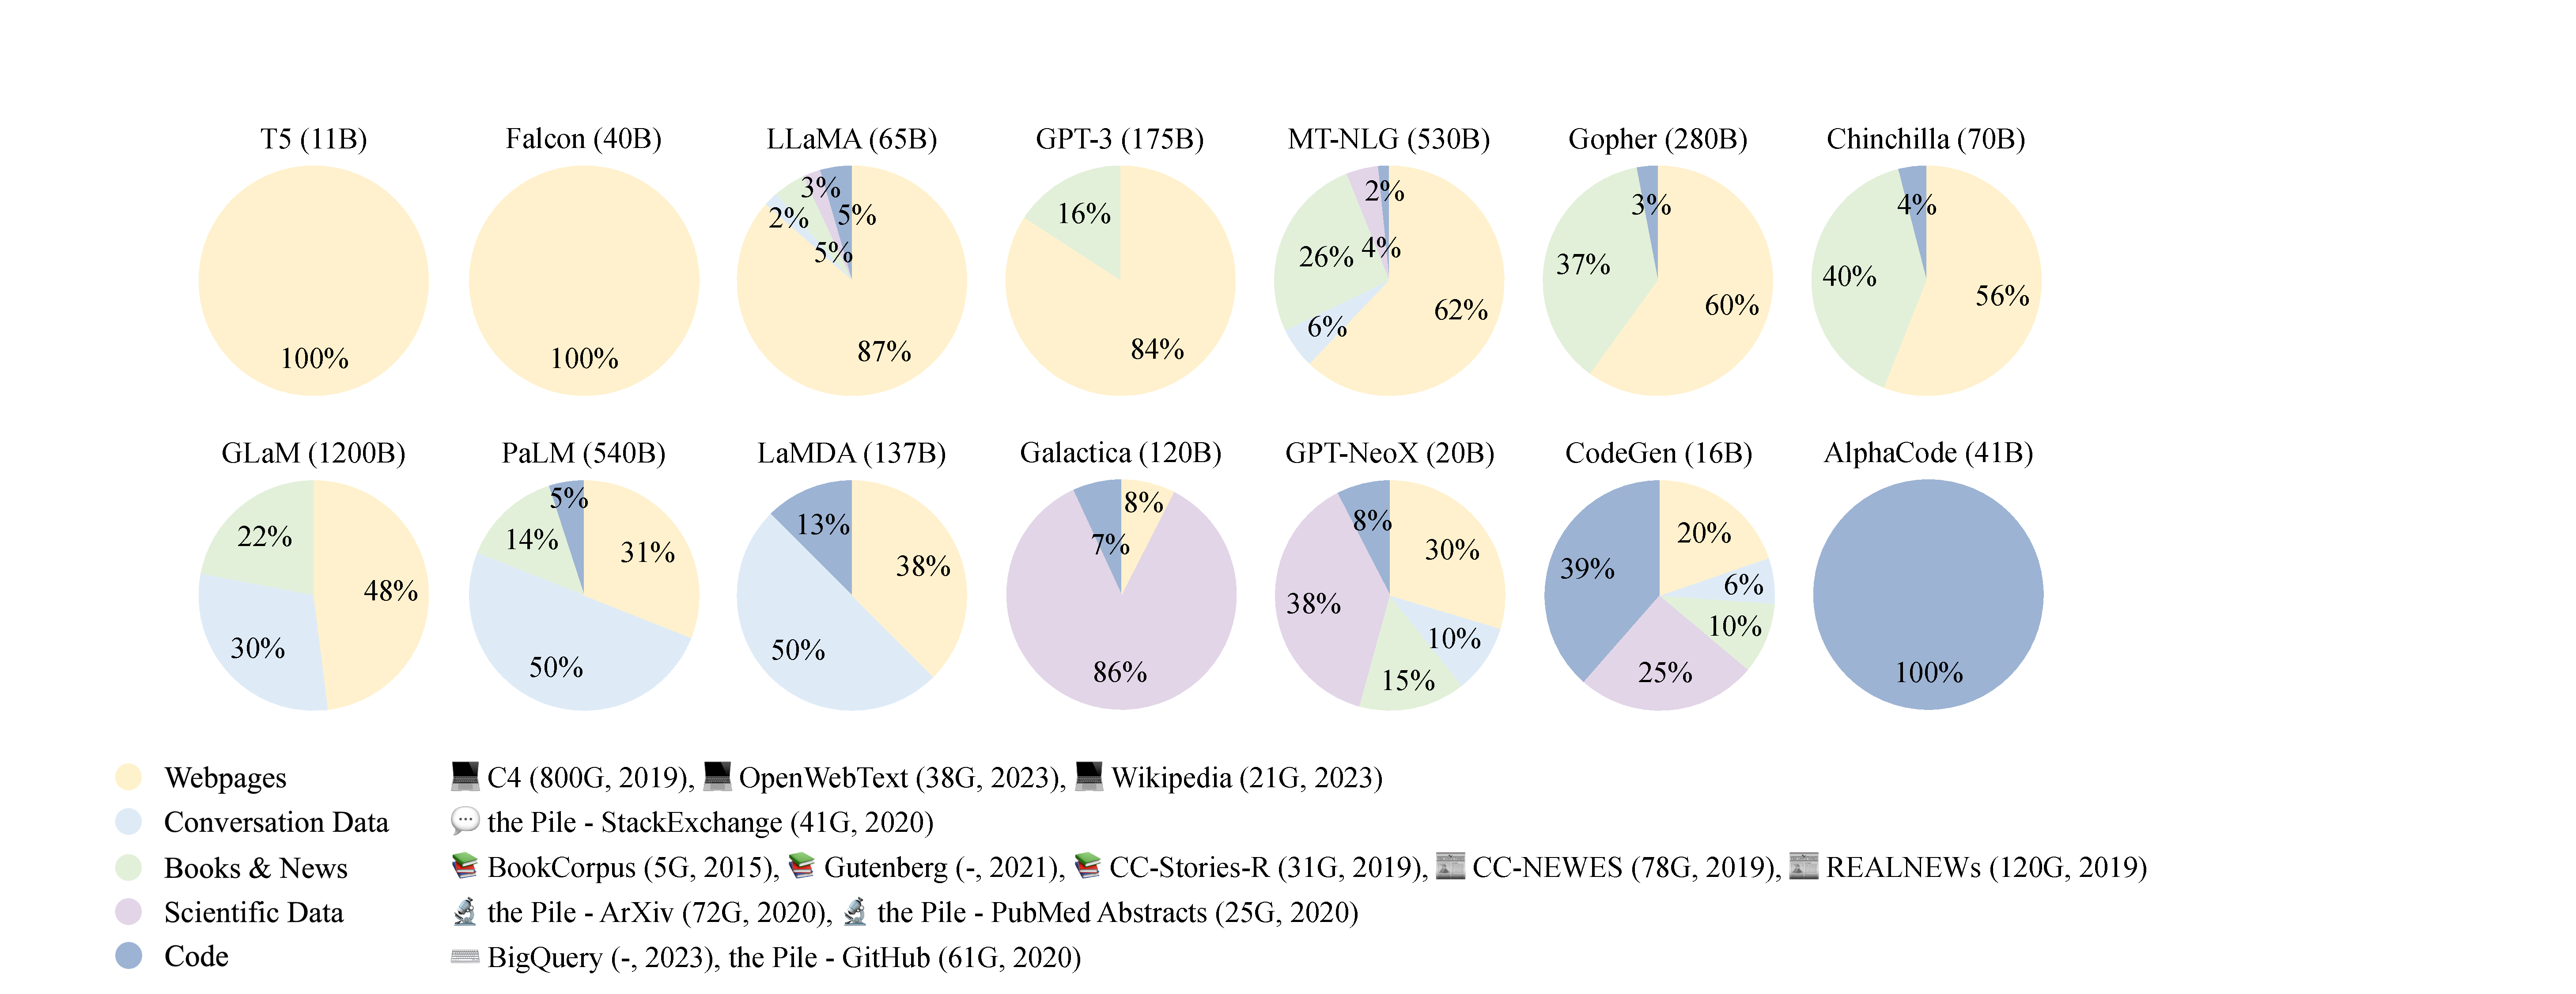
\includegraphics[width=\textwidth]{images/source_ratio_1009.pdf}
    \caption{Ratios of various data sources in the pre-training data for existing  LLMs. }
    \label{fig:source-ratio}
\end{figure*}

\section{Pre-training}
\label{sec-pretraining}

Pre-training establishes the basis of the abilities of LLMs. By pre-training on large-scale corpora, LLMs can acquire essential language understanding and %
{generation} skills~\cite{Brown-NeurIPS-2020-Language,Chowdhery-arxiv-2022-PaLM}.
In this process, the scale and quality of the pre-training corpus are critical for LLMs to attain powerful capabilities.
Furthermore, to effectively pre-train LLMs,  model architectures, acceleration methods, and optimization techniques need to be well designed. In what follows, we  first discuss the data collection and processing in Section~\ref{sec:data_collection}, then introduce the commonly used model architectures in Section~\ref{sec:architecture}, and finally present the training techniques to stably and efficiently  optimize LLMs in Section~\ref{sec:training_settings}.

\subsection{Data Collection and Preparation}
\label{sec:data_collection}
Compared with small-scale language models, LLMs have a stronger demand for high-quality data for model pre-training, and their model capacities  largely rely on the pre-training corpus and how it has been preprocessed. In this part, we discuss the collection and processing of pre-training data, including data sources, preprocessing methods, and important analysis of how pre-training data affects the performance of LLMs.


\subsubsection{Data Source}\label{sec-source}
To develop a capable LLM, it is key to collect a large amount of natural language corpus from various data sources.
Existing LLMs mainly leverage a mixture of diverse public textual datasets as the pre-training corpus. 
Figure~\ref{fig:source-ratio} shows  the distribution of the sources of pre-training data for a number of representative LLMs. 

The source of pre-training corpus can be broadly categorized into two types: general data and specialized data. General data, such as webpages, books, and conversational text, is utilized by most LLMs~\cite{Chowdhery-arxiv-2022-PaLM,Brown-NeurIPS-2020-Language,Zhang-arxiv-2022-OPT} due to its large, diverse, and accessible nature, which can enhance the language modeling and generalization abilities of LLMs. In light of the impressive generalization capabilities exhibited by LLMs, there are also studies that extend their pre-training corpus to more specialized datasets, such as multilingual data, scientific data, and code, endowing LLMs with specific task-solving capabilities~\cite{Chowdhery-arxiv-2022-PaLM,Taylor-arxiv-2022-Galactica, nijkamp-arxiv-2022-Codegen}. In what follows, we describe these two types of pre-training data sources and their effects on LLMs.  {For a detailed introduction to the commonly used corpus, one can refer to Section~\ref{sec:commonly_used_corpora}.} 

\paratitle{General Text Data.}
As we can see in Figure~\ref{fig:source-ratio}, the vast majority of LLMs adopt general-purpose pre-training data, such as webpages, books, and conversational text, which provides rich text sources on a variety of topics. 
Next, we briefly summarize three important kinds of general data.

$\bullet$ \emph{Webpages.} Owing to the proliferation of the Internet, various types of data have been created, which enables LLMs to gain diverse linguistic knowledge and enhance their generalization capabilities~\cite{radford-blog-2019-language,Raffel-JMLR-2020-Exploring}. For convenient use of these data resources, a large amount of data is crawled from the web in previous work, such as CommonCrawl~\cite{commoncrawl}. However, the crawled web data tends to contain both high-quality text, such as Wikipedia and low-quality text, like spam mail, thus it is important to filter and process webpages for improving the data quality. 

$\bullet$ \emph{Conversation text.} %
Conversation data can enhance the conversational competence of LLMs~\cite{Zhang-arxiv-2022-OPT} and potentially improve their performance on a range of question-answering tasks~\cite{Chowdhery-arxiv-2022-PaLM}. 
Researchers can utilize  subsets of public conversation corpus (\eg PushShift.io Reddit corpus)~\cite{Roller-ACL-2021-Recipes,Baumgartner-AAAI-2020-The} or collect conversation data from online social media.  
{Since online conversational data often involves discussions among multiple participants, an effective processing way  is to transform a conversation into a tree structure, where the utterance is linked to the one it responds to.
In this way, the multi-party conversation tree can be divided into multiple sub-conversations, which can be collected in the pre-training corpus.}
Furthermore, a potential risk is that the excessive integration of dialogue data into LLMs may result in a side effect~\cite{Zhang-arxiv-2022-OPT}:  declarative instructions and direct interrogatives are erroneously perceived as the beginning of conversations, thus leading to a decline in the efficacy of the instructions. 

$\bullet$ \emph{Books.} Compared to other corpus, books provide an important source of  formal long texts, which are potentially   beneficial for %
{LLMs to learn  linguistic knowledge, model long-term dependency, and generate narrative and coherent texts.}
To obtain open-source book data, existing studies usually adopt the Books3 and Bookcorpus2 datasets, which are available in the Pile dataset~\cite{Gao-arxiv-2021-Pile}. 

\paratitle{Specialized Text Data.} Specialized  datasets are  useful to improve the specific capabilities of LLMs on downstream tasks.  
Next, we introduce three kinds of specialized data.

$\bullet$ \emph{Multilingual text.}  
In addition to the text in the target language, 
integrating a multilingual corpus can enhance the multilingual abilities of language understanding and generation. 
 For example, BLOOM~\cite{Scao-arxiv-2022-BLOOM} and PaLM~\cite{Chowdhery-arxiv-2022-PaLM} have curated multilingual data covering 46 and 122 languages, respectively, within their pre-training corpora. FLM~\cite{Li-arxiv-2023-FLM} mixes Chinese and English corpora in nearly equal proportions. These models demonstrate impressive performance in multilingual tasks, such as translation, multilingual summarization, and multilingual question answering, and achieve comparable or superior performance to the state-of-the-art models that are fine-tuned on the corpus in the target language(s).


$\bullet$ \emph{Scientific text.}
The exploration of science by humans has been witnessed by the increasing growth  of scientific publications. 
In order to enhance the understanding of scientific knowledge for LLMs~\cite{Taylor-arxiv-2022-Galactica,Lewkowycz-arxiv-2022-Solving}, 
it is useful to incorporate a scientific corpus for model pre-training~\cite{Taylor-arxiv-2022-Galactica,Lewkowycz-arxiv-2022-Solving}. %
By pre-training on a vast amount of scientific text, LLMs can achieve impressive performance in scientific and reasoning tasks~\cite{Saier-arxiv-2023-unarXive}.
To construct the scientific corpus, existing efforts mainly collect arXiv papers, {scientific textbooks}, math webpages, and other related scientific resources.  
 Due to the complex nature of data in scientific fields, such as mathematical symbols and protein sequences, specific tokenization and preprocessing techniques are usually required to transform these different formats of data into a unified form that can be processed by language models.

$\bullet$ \emph{Code.} Program synthesis has been widely studied in the research community~\cite{Simon-JACM-1963-Experiments,Manna-CommunACM-1971-Toward,Feng-EMNLPFindings-2020-CodeBERT,Chen-arxiv-2021-evaluating,Austin-arxiv-2021-Program}, especially the use of PLMs trained on code~\cite{Black-GitHub-2021-GPT-Neo,Wang-GitHub-2021-GPT-J}.   
However, it remains challenging for these PLMs (\eg GPT-J~\cite{Wang-GitHub-2021-GPT-J}) to generate high-quality and accurate programs.
Recent studies~\cite{Chen-arxiv-2021-evaluating,Austin-arxiv-2021-Program} have found that training LLMs  on a vast code corpus can lead to a substantial improvement in the quality of the synthesized programs. The generated programs can successfully pass expert-designed unit-test cases~\cite{Chen-arxiv-2021-evaluating} or solve competitive programming questions~\cite{Li-Science-2022-AlphaCode}. %
{In general, two types of code corpora are commonly used for pre-training LLMs. The first source is  from programming question answering  communities like Stack Exchange~\cite{Xu-SIGPLAN-2022-Systematic}. The second source is  from public software repositories such as GitHub~\cite{Chen-arxiv-2021-evaluating,Austin-arxiv-2021-Program,nijkamp-arxiv-2022-Codegen}, where code data (including comments and docstrings)  are collected for utilization.}
Compared to natural language text, code is  in the format of a programming language, corresponding to long-range  dependencies and accurate execution logic~\cite{Madaan-emnlp-2022-Language}. 
{A recent study~\cite{FU-blog-2022-how}} also speculates that training on code might be a source of complex reasoning abilities (\eg chain-of-thought ability~\cite{Wei-arxiv-2022-chain}).  
{Furthermore, it has been shown that  formatting reasoning tasks into code can help  LLMs generate more accurate results~\cite{Madaan-emnlp-2022-Language}.}









\subsubsection{Data Preprocessing}
\label{sec:data_pre_processing}
After collecting a large amount of text data, it is essential to preprocess the data for constructing  the pre-training corpus, especially removing  noisy, redundant, irrelevant, and potentially toxic data~\cite{Rae-arxiv-2021-Scaling, Chowdhery-arxiv-2022-PaLM, Longpre-arxiv-2023-pretrainer}, which may largely affect the  capacity and performance of LLMs.  
{To facilitate the data processing, 
a recent study~\cite{Chen-2023-arxiv-Data} proposes a useful data processing system for LLMs, named Data-Juicer, which provides over 50 processing operators and tools.}
In this part, we review the detailed data preprocessing strategies to improve the quality of the collected data~\cite{Rae-arxiv-2021-Scaling,Du-ICML-2022-GLaM,Scao-arxiv-2022-BLOOM}. 
{A typical pipeline of preprocessing the pre-training data for LLMs has been illustrated in Figure~\ref{fig:processing-pipeline}.}

\begin{figure*}
    \centering
    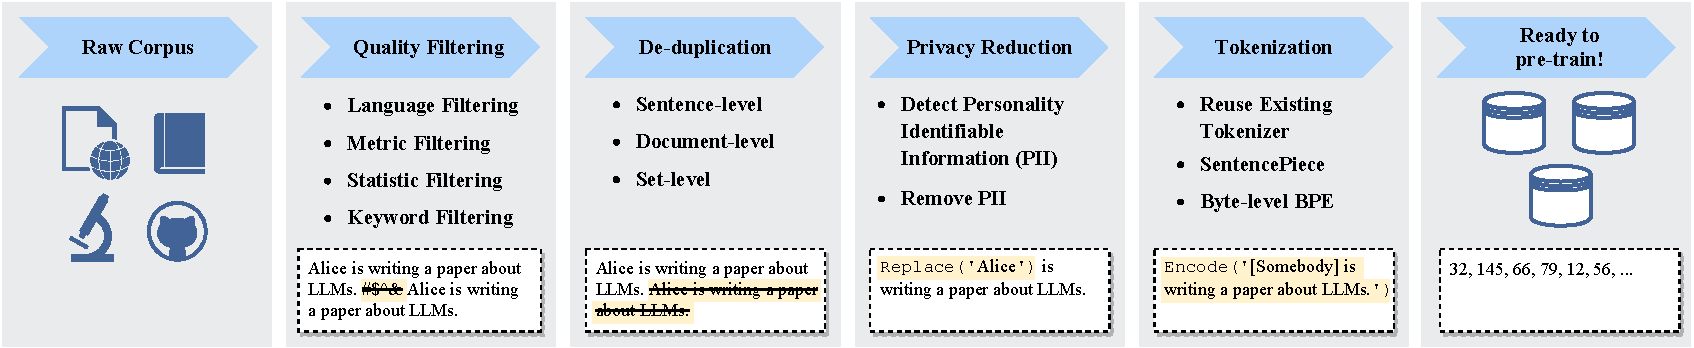
\includegraphics[width=1\textwidth]{images/pipeline_0331.pdf}
    \caption{An illustration of a typical data preprocessing pipeline for pre-training large language models. }
    \label{fig:processing-pipeline}
\end{figure*}


\paratitle{Quality Filtering.}
To remove low-quality data from the collected corpus, existing work generally adopts two approaches: (1) classifier-based, and (2) heuristic-based. 
The former approach  trains a selection classifier based on high-quality texts and leverages it to identify and filter out low-quality data. 
Typically, these methods~\cite{Brown-NeurIPS-2020-Language,Du-ICML-2022-GLaM,Chowdhery-arxiv-2022-PaLM} train a binary classifier with well-curated data (\eg Wikipedia pages) as positive instances and sample candidate data as negative instances, and predict the score that measures  the quality of each data  example. 
However, several studies~\cite{Du-ICML-2022-GLaM, Rae-arxiv-2021-Scaling} find that a classifier-based approach may result in the unintentional removal of high-quality texts in dialectal, colloquial, and sociolectal languages, which potentially leads to bias in the pre-training corpus and diminishes the corpus diversity.
As the second approach, several studies, such as BLOOM~\cite{Scao-arxiv-2022-BLOOM} and Gopher~\cite{Rae-arxiv-2021-Scaling}, employ heuristic-based approaches to eliminate low-quality texts through a set of well-designed rules, which can be summarized as follows:

\begin{itemize}[leftmargin=0.5cm, itemsep=5pt]
\item \emph{Language based filtering.} If a LLM would  be mainly used  in the tasks of certain languages, the text in other languages can be filtered.

\item \emph{Metric based filtering.} Evaluation metrics about the generated texts, \eg perplexity, can be employed to detect and remove unnatural sentences.

\item \emph{Statistic based  filtering.} Statistical features of a corpus, \eg the punctuation distribution, symbol-to-word ratio, and sentence length, can be utilized to measure the text quality and filter the low-quality data.

\item \emph{Keyword based filtering.} Based on specific keyword set, the noisy or unuseful elements in the text, such as HTML tags, hyperlinks, boilerplates, and offensive words, can be identified and removed. 
\end{itemize}

\paratitle{De-duplication.}
Existing work~\cite{Hernandez-arxiv-2022-Scaling} has found that duplicate data in a corpus would reduce the diversity of language models, which may  cause the training process to become unstable and thus affect the model performance.
Therefore, it is necessary to de-duplicate the pre-training corpus. 
Specially, de-duplication can be performed at different granularities, including sentence-level, document-level, and dataset-level de-duplication. 
First,  low-quality sentences that contain repeated words and phrases should be removed,  as they may introduce repetitive patterns in language modeling~\cite{Holtzman-2019-ICLR-The}. At the document level, existing studies mostly rely on the overlap ratio of surface features (\eg words and $n$-grams overlap) between documents to detect and remove duplicate documents containing similar contents~\cite{Rae-arxiv-2021-Scaling,Touvron-arxiv-2023-LLaMA,Scao-arxiv-2022-BLOOM,Lee-ACL-2022-Deduplicating}. 
Furthermore, to avoid the dataset contamination problem, it is also crucial to prevent the overlap between the training and evaluation sets~\cite{Chowdhery-arxiv-2022-PaLM}, by removing the possible duplicate texts  from the training set.
It has been shown that the three levels of de-duplication are useful to improve the training of LLMs~\cite{Carlini-arxiv-2022-Quantifying,Chowdhery-arxiv-2022-PaLM}, which should be jointly used in practice. 

\paratitle{Privacy Reduction.} 
The majority of pre-training text data is obtained from web sources, including user-generated content involving sensitive or personal information, which may increase the risk of privacy breaches~\cite{Carlini-USENIX-2021-Extracting}. 
Thus, it is necessary to remove the \emph{personally identifiable information~(PII)}  from the pre-training corpus. One direct and effective approach is to employ rule-based methods, such as keyword spotting, to detect and remove PII such as names, addresses, and phone numbers~\cite{Laurencon-NIPS-2022-The}. Furthermore, researchers also find that the vulnerability of LLMs under privacy attacks can be attributed to the presence of {duplicate PII data} in the pre-training corpus~\cite{Kandpal-ICML-2022-Deduplicating}. Therefore, de-duplication can also reduce privacy risks to some extent.

\paratitle{Tokenization.}
Tokenization is also a crucial step for data preprocessing.  
It aims to segment raw text into sequences of individual tokens, which are subsequently used as the inputs of LLMs. In traditional NLP research (\eg sequence labeling with conditional random fields~\cite{Lafferty-ICML-2001}), word-based tokenization is the predominant approach, which is more aligned with human's language cognition. However, word-based tokenization can yield different segmentation results for the same input in some languages (\eg Chinese word segmentation), generate  a huge word vocabulary containing many low-frequency words, and also suffer from the ``\emph{out-of-vocabulary}'' issue. Thus, several  neural network models employ \emph{character} as the minimum unit to derive the word representation (\eg a CNN word encoder in ELMo~\cite{Peters-NAACL-2018}). Recently, \emph{subword tokenizers} have been widely used in Transformer based language models, typically including Byte-Pair Encoding tokenization, WordPiece   tokenization and Unigram tokenization. HuggingFace has maintained an excellent online NLP course  on tokenizer\footnote{https://huggingface.co/learn/nlp-course/chapter6} with running examples, and we refer to the beginners to this course. Next, we briefly describe the three representative  tokenization methods. 

$\bullet$ \emph{Byte-Pair Encoding~(BPE) tokenization}. BPE was originally proposed as a general data compression algorithm in 1994~\cite{Philip-1994-BPE}, and then adapted to NLP for tokenization~\cite{Sennrich-ACL-2016-nueral}. It starts with a set of basic symbols (\eg the alphabets and boundary characters), and iteratively combine frequent pairs of two consecutive tokens in the corpus as new tokens (called \emph{merge}). For each merge, the selection criterion is based on the co-occurrence frequency of two   contiguous tokens: the top frequent pair would be selected. The merge process continues until it reaches the predefined size.  
Further, Byte-level BPE has been used  to improve the tokenization quality for multilingual corpus (\eg the text containing non-ASCII characters) by considering \emph{bytes} as the basic symbols for merge. %
Representative language models with this tokenization approach include GPT-2, BART, and LLaMA. 


$\bullet$ \emph{WordPiece tokenization}.  WordPiece was a Google internal subword tokenization algorithm. 
It was originally proposed by Google in developing voice search systems~\cite{Mike-ICASSP-2012-Japanese}. Then, it was  used in the neural machine translation system in 2016~\cite{Wu-CoRR-2016}, and  was adopted as the word tokenizer for BERT in 2018~\cite{Devlin-NAACL-2019-BERT}.  WordPiece has a very similar idea with BPE by iteratively merging consecutive tokens, whereas taking a slightly different  selection criterion for the merge. To conduct the merge, it first trains a language model and  employs it to score all possible pairs. Then, at each merge, it selects the pair that leads to the most increase in the likelihood of training data. 
Since Google has't released the official implementation of the WordPiece algorithm, HuggingFace gives a more intuitive selection measure  in its online NLP course: a pair is scored by dividing the co-occurrence count by the product of the occurrence counts of two tokens in the pair based on training corpus. 

$\bullet$ \emph{Unigram tokenization}.
Unlike BPE and WordPiece, Unigram tokenization~\cite{Kudo-ACL-2018-Subword} starts with a sufficiently large set of  possible substrings or subtokens for a corpus, and iteratively removes the tokens in the current vocabulary until the expected vocabulary size is reached. 
As the selection criterion, it calculates  the yielded increase in the likelihood of training corpus by assuming that some token was removed from current vocabulary.  
This step is conducted based on a trained unigram language model. To estimate the unigram language model, it adopts 
an expectation–maximization~(EM) algorithm: at each iteration, we first find the currently optimal tokenization of words based on the old language model, and then re-estimate the probabilities of unigrams to update the language model. During this procedure, dynamic programming algorithms (\ie the Viterbi algorithm) are  used to efficiently find the optimal decomposition way of a word given the language model. 
Representative models that adopt this tokenization approach include T5 and mBART. 

%



Although it is expedient to leverage an existing tokenizer (\eg OPT~\cite{Zhang-arxiv-2022-OPT} and GPT-3~\cite{Brown-NeurIPS-2020-Language} utilize the tokenizer of GPT-2~\cite{radford-blog-2019-language}), using a  tokenizer specially designed for the pre-training corpus can be highly beneficial~\cite{Scao-arxiv-2022-BLOOM}, especially for the corpus that consists of diverse domains, languages, and {formats}. 
{Therefore, recent LLMs often train the customized tokenizers specially for the  pre-training corpus with the SentencePiece library~\cite{Kudo-EMNLP-2018-SentencePiece}, which includes Byte-level BPE and Unigram tokenization. 
{A note is that normalization techniques in BPE, such as NFKC~\cite{Davis-arxiv-2001-Unicode}, may  degrade the tokenization performance~\cite{Hoffmann-arxiv-2022-Training,Rae-arxiv-2021-Scaling,Scao-arxiv-2022-BLOOM}. } 
When extending existing LLMs  (\ie continual pre-training or instruction tuning), we should be also aware of the potential side effect with customized tokenizers.   
For example, LLaMA trains  
the BPE tokenizer  based on a pre-training corpus mainly consisting of English texts, and the derived vocabulary might be less capable in processing non-English data, \eg taking longer inference latency to generate Chinese texts. 

\paratitle{Discussion on Effect of Data Quality.} %
{For pre-training, the quality of pre-training data is vital to the  model capacities of LLMs. %
Existing work has shown that pre-training on the low-quality corpus, such as noisy, toxic, and duplicate data, would largely hurt the performance of models~\cite{Rae-arxiv-2021-Scaling, Lee-ACL-2022-Deduplicating, Kandpal-ICML-2022-Deduplicating, Hernandez-arxiv-2022-Scaling}.
Recent studies, such as T5~\cite{Raffel-JMLR-2020-Exploring}, GLaM~\cite{Du-ICML-2022-GLaM}, and Gopher~\cite{Rae-arxiv-2021-Scaling}, have investigated the influence of data quality on the LLMs' capacities.
By comparing the performance of models trained on the filtered and unfiltered corpus, they have reached the similar conclusion that pre-training LLMs on cleaned data can improve the model performance.  %
More specifically, the duplication of data may result in ``\emph{double descent}'' (referring to the phenomenon of performance initially deteriorating and subsequently improving)~\cite{Hernandez-arxiv-2022-Scaling,Nakkiran-ICLR-2020-Deep}, or even overwhelm the training process~\cite{Hernandez-arxiv-2022-Scaling}. 
In addition, it has been shown that duplicate data degrades the ability of LLMs to copy from the context, which might further affect the generalization capacity of LLMs using in-context learning~\cite{Hernandez-arxiv-2022-Scaling}.
Therefore, as suggested in~\cite{Rae-arxiv-2021-Scaling, Scao-arxiv-2022-BLOOM, Chowdhery-arxiv-2022-PaLM, Longpre-arxiv-2023-pretrainer}, {it is essential to utilize  preprocessing methods like quality filtering, toxic filtering and deduplication to carefully clean  the pre-training corpus  (as illustrated in Section~\ref{sec:data_pre_processing}), } to improve stability of the training process and avoid affecting the model performance.
}


\begin{figure}
    \centering
    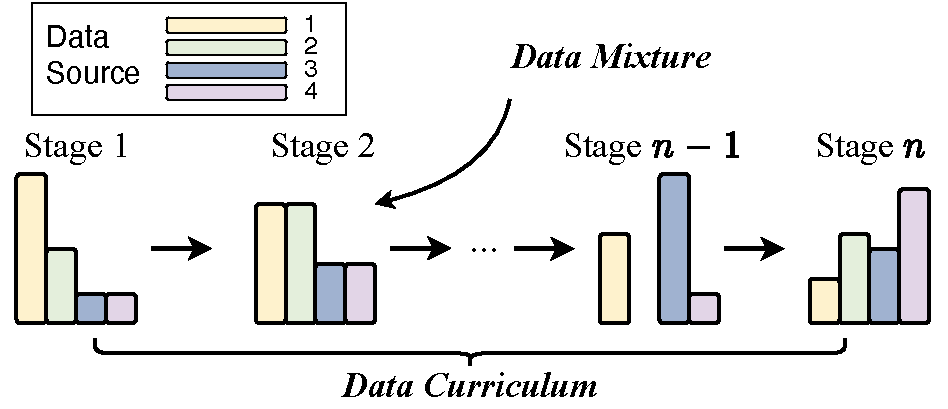
\includegraphics[width=0.48\textwidth]{images/data_schedule.pdf}
    \caption{An illustration of  data scheduling for pre-training LLMs. }
    \label{fig:data_schedule}
\end{figure}

\subsubsection{Data Scheduling}
\label{sec:data_scheduling}
After data preprocessing, it is essential to design suitable strategies to schedule these multi-source data  for pre-training a capable LLM. Generally, two key aspects should be paid close attention for data scheduling: the proportion of each data source (\emph{data mixture}), and the order in which each data source is scheduled for training (\emph{data curriculum}).
Next, we discuss the two aspects in detail. An illustration of data scheduling has been presented in Figure~\ref{fig:data_schedule}.

\paratitle{Data Mixture.}
 Since each kind of data source is closely related to the development of certain capacities for  LLMs (referring to the discussions in Section~\ref{sec:data_collection}), it is important to set a suitable  distribution to mix these data. 
 The data mixture is generally set in a global level (\ie the distribution of the entire pre-training data), and can be also locally set to varied  proportions at different training stages. 
 During pre-training, data samples from different sources would be selected according to the mixture proportions: more data will be sampled from a data source with a larger weight.  
Typically, existing LLMs such as LLaMA~\cite{Touvron-arxiv-2023-LLaMA} may employ upsampling or downsampling on the full data of each source to create specific data mixtures as pre-training data. 
As Figure~\ref{fig:source-ratio} illustrates, existing LLMs use different data mixtures to construct the pre-training data.  
As a representative model, the pre-training data of LLaMA~\cite{Touvron-arxiv-2023-LLaMA} mainly consists of webpages (over 80\%),  alongside 6.5\% of code-heavy data from GitHub and StackExchange, 4.5\% from books, and 2.5\% of scientific data sourced from arXiv, which has become an important reference for training  general-purpose LLMs. 
Furthermore, special data mixtures can be used to facilitate different   purposes. For example,  Falcon~\cite{Penedo-2023-arxiv-Refinedweb} is trained on pure webpages,   and CodeGen~\cite{nijkamp-arxiv-2022-Codegen} largely increases the amount of code data. 
In practice, data mixture is often determined empirically, and we summarize several common strategies for finding an effective data mixture as follows: 


{$\bullet$ \emph{Increasing the diversity of data sources.}
Recent studies have empirically shown that training on excessive data about a certain domain would degrade the generalization capability of LLMs on other domains~\cite{Taylor-arxiv-2022-Galactica,Rae-arxiv-2021-Scaling}. In contrast, increasing the data source heterogeneity (\eg  including diverse data sources) is critical for improving the downstream performance of LLMs~\cite{Longpre-arxiv-2023-pretrainer,Tirumala-2023-arXiv-D4,Shen-2023-arXiv-SlimPajamaDC}. 
To further examine the effect of different data sources, some studies  have conducted ablation experiments by removing  each data source one by one,  and pre-train LLMs with specially curated datasets~\cite{Longpre-arxiv-2023-pretrainer}. It has been shown  that dropping data sources with high heterogeneity (\eg webpages) impacts LLM's abilities more severely than dropping sources with low heterogeneity (\eg academic corpus).
}

{$\bullet$ \emph{Optimizing data mixtures.}
In addition to manually setting the data mixtures, several studies have proposed to optimize the data mixtures for improving the model pre-training~\cite{Xie-arxiv-2023-DSIR,Xie-arxiv-2023-doremi}. Given the target downstream tasks, one can select pre-training data with either higher proximity in the feature space~\cite{Xie-arxiv-2023-DSIR} or those that provide positive influences on downstream  task performance~\cite{Wang-2023-arXiv-farewell}. %
Further, to reduce the reliance of target tasks, DoReMi~\cite{Xie-arxiv-2023-doremi} %
 first trains a small reference model using   given initial domain weights, and then trains another small proxy model, upweighting the domains   on which the greatest discrepancies in  likelihood between the two models are observed. Finally, the learned  domain weights of the proxy model are applied to train a much larger LLM.} 
In a more simple way, one can train several small  language models with different data mixtures, and select the data mixture that leads to  the most desirable performance.
However, an assumption made in this  approach is,   when trained in a similar way,  small models would resemble with large models in model abilities or behaviors, which may not always hold in practice. 
}

{$\bullet$ \emph{Specializing the targeted abilities.} 
The model capacities of LLMs heavily rely on data selection and mixture, and one can boost the proportions of specific data sources to enhance certain model abilities~\cite{Rae-arxiv-2021-Scaling,Longpre-arxiv-2023-pretrainer}.  
For example,   
 the mathematical reasoning and coding abilities can be specially enhanced by training with more mathematical texts and code data, respectively. 
Furthermore, experimental results on the LAMBADA dataset~\cite{Paperno-ACL-2016-LAMBADA} show that increasing the proportion of books data can improve the model capacity  in capturing long-term dependencies from text, and increasing the proportion of the C4 dataset~\cite{Raffel-JMLR-2020-Exploring} leads to performance improvement on the C4 validation dataset~\cite{Rae-arxiv-2021-Scaling}.  
Generally, it is important to identify more implicit relations between data sources and  model abilities. {
To enhance specific skills such as mathematics and coding in LLMs, or to develop specialized LLMs, a practical way is to employ a multi-stage training approach, \eg general and skill-specific data can be  scheduled at two consecutive stages. This approach of training LLMs on varying sources or proportions of data across multiple stages is also known as ``data curriculum'', which will be introduced below.   
}

\paratitle{Data Curriculum.} 
{
After preparing the data mixture, it is important to schedule the order that specific data is presented to LLMs for pre-training. 
It has been shown that, in some cases, to learn a certain skill, learning in a skill-set sequence (\eg basic skills $\rightarrow$ target skill) outperforms direct learning from a corpus focused solely on the target skill~\cite{Chen-2023-arXiv-skill,Roziere-arxiv-2023-codellama}. 
Following the idea of curriculum learning~\cite{Bengio-2009-arXiv-curriculum}, \emph{data curriculum} has been proposed and widely used in model pre-training~\cite{Chen-2023-arXiv-skill,Xu-2023-arXiv-contrastive,Roziere-arxiv-2023-codellama,Tworkowski-arxiv-2023-Focused}. It aims to  organize different parts of pre-training data for LLMs in a specific order, \eg  starting  with easy/general examples and progressively introducing  more challenging/specialized ones. 
More generally, 
it can broadly refer to the adaptive adjustment of data proportions for different sources during pre-training. 
Existing work about  data curriculum mainly focuses on continual pre-training, such as specialized coding LLMs (\eg CodeLLaMA~\cite{Roziere-arxiv-2023-codellama}) or long context LLMs (\eg LongLLaMA~\cite{Tworkowski-arxiv-2023-Focused}).
However, it still lacks of more detailed report about data curriculum for general-purpose LLMs (\eg LLaMA) in the literature. 
To determine data curriculum, a practical approach is to monitor the development of key abilities of LLMs based on specially constructed evaluation benchmarks, and then adaptively adjust the data mixture during pre-training. 
Next, we take  three common abilities as examples to introduce how the concept of data curriculum\footnote{We utilize the symbol ``$\rightarrow$'' to represent the data order  in  data curriculum. For example, ``2T webpage  tokens $\rightarrow$ 500B code tokens'' means that the LLM is firstly trained with 2T webpage tokens and subsequently with 500B code data tokens. } applies in continual pre-training. 
}


{
$\bullet$ \emph{Coding}. To improve the coding ability of LLMs, CodeLLaMA~\cite{Roziere-arxiv-2023-codellama} is developed based on LLaMA 2~\cite{Touvron-2023-llama2-arxiv}
(2T general tokens $\rightarrow$ 500B code-heavy tokens), aiming to improve the code generation ability and retain natural language understanding skills.   CodeLLaMA also provides a version that is further specialized to a certain programming language, namely CodeLLaMA-Python (2T general tokens $\rightarrow$ 500B code-heavy tokens $\rightarrow$ 100B Python-heavy tokens).
}

{
$\bullet$ \emph{Mathematics.} Llemma~\cite{Azerbayev-arxiv-2023-llemma} is proposed to enhance the mathematical capacities of general-purpose LLMs.
It is developed based on CodeLLaMA. 
Although CodeLLaMA~\cite{Roziere-arxiv-2023-codellama} mainly focuses on the coding ability, experiments have shown that it performs better than its base model LLaMA 2 on mathematics benchmarks~\cite{Azerbayev-arxiv-2023-llemma}. %
Based on CodeLLaMA, Llemma is continually trained on mixtures of scientific papers, web data containing mathematical text and  code (2T general tokens $\rightarrow$ 500B code-heavy tokens $\rightarrow$ 50$\sim$200B math-heavy tokens). Note that the pre-training data of Llemma also contains 5\% general domain data as a form of regularization.
}

{
$\bullet$ \emph{Long context}. Long context modeling is an important ability for LLMs, and  many studies have explored extending the  context windows of LLMs via continually training~\cite{Roziere-arxiv-2023-codellama,Tworkowski-arxiv-2023-Focused}. With modifications on position embeddings (\ie  position interpolation) of RoPE-based LLMs~\cite{Touvron-2023-llama2-arxiv,Touvron-arxiv-2023-LLaMA,Chen-arxiv-2023-Extending}, 
CodeLLaMA further extends the context window of LLaMA 2 (2.5T tokens with 4K context window $\rightarrow$ 20B tokens with 16K context window).
LongLLaMA~\cite{Tworkowski-arxiv-2023-Focused} also achieves longer context window 
with the help of external memory and a unique training objective (1T tokens with 2K context window $\rightarrow$ 10B tokens with 8K context window).
}








%

{
\subsubsection{Summary of Data Preparation}
\label{sec:data_prepare_sug}
In this part, we summarize the general procedure and key points  to prepare pre-training data for LLMs, which are  detailed in the following three aspects.    
}

{
$\bullet$ \emph{Data collection.} It is suggested to include  diverse data sources in  the pre-training data.  Although Falcon~\cite{Penedo-2023-arxiv-Refinedweb} shows that webpages alone can be employed to train powerful LLMs, a more typical approach is to also incorporate  diverse high-quality text like code, books, scientific papers, \etc.
If a LLM is specialized with a certain skill, the proportion of corresponding data source should be increased accordingly.  %
For example, Gopher~\cite{Rae-arxiv-2021-Scaling} and Chinchilla~\cite{Hoffmann-arxiv-2022-Training} are trained with approximately 40\% of data from books. PaLM~\cite{driess-arxiv-2023-palm} and LaMDA~\cite{Thoppilan-CoRR-2022-LaMDA} use  approximately 50\% conversational data.
}

{
$\bullet$ \emph{Data cleaning.} After data collection, it is crucial to clean the raw corpus to enhance its quality as possible. First, deduplication is commonly  used in existing work~\cite{Touvron-2023-llama2-arxiv,Tirumala-2023-arXiv-D4,Penedo-2023-arxiv-Refinedweb}.
Second,  low-quality text, toxic content, and data with privacy concerns should be removed at different granularities (\eg document, passage or sentence). In practice,  both heuristic and classifier-based methods can be employed for quality and toxicity filtering (\eg CCNet~\cite{Wenzek-2020-LREC-CCNet}, fastText~\cite{Joulin-2017-EACL-fasttext}, and Data-Juicer~\cite{chen-2023-arXiv-DataJuicer}). Third,  with the cleaned data, one can further unify or specify the  format for pre-training data, and perform the tokenization by training the tokenizer on the filtered and deduplicated corpus with libraries like SentencePiece~\cite{Kudo-EMNLP-2018-SentencePiece}. 
}

{
$\bullet$ \emph{Data scheduling.} %
With the preprocessed data, the next step is to determine the data mixture and the specific order of data for pre-training LLMs.  
To determine both settings, a practical way is to first train several small  language models with multiple candidate plans and then select a good plan among them~\cite{Xie-arxiv-2023-doremi}.
Overall, it is more difficult to find a  suitable data curriculum. 
In practice, one can monitor the performance of intermediate model checkpoints on specific evaluation benchmarks, and dynamically tune the data mixture and distribution during  pre-training. In this process, it is also useful to explore the potential relations between data sources and model abilities to instruct the design of data curriculum. 
}












\subsection{Architecture}
\label{sec:architecture}
 In this section, we review the architecture design  of LLMs, \ie mainstream architecture, pre-training objective, and detailed configuration. Table~\ref{model_card}  presents the model cards of several representative LLMs with public details.  


\begin{table*}[htb]
    \centering
    \caption{Model cards of several selected  LLMs with public configuration details. Here, PE denotes position embedding, \#L denotes the number of layers, \#H denotes the number of attention heads, $d_{model}$ denotes the size of hidden states, and MCL denotes the maximum context length during training.}
    \begin{tabular}{lcrccccrrrr}
    \toprule
         \textbf{Model}&\textbf{Category}&\textbf{Size}&\textbf{Normalization}&\textbf{PE}&\textbf{Activation}&\textbf{Bias}&\textbf{\#L}&\textbf{\#H}&\textbf{$d_{model}$}&\textbf{MCL} \\
\midrule
GPT3~\cite{Brown-NeurIPS-2020-Language}&Causal decoder&175B&Pre LayerNorm&Learned&GeLU&\checkmark&96&96&12288&2048\\
PanGU-~$\alpha$~\cite{Zeng-arxiv-2021-PanGualpha}&Causal decoder&207B&Pre LayerNorm&Learned&GeLU&\checkmark&64&128&16384&1024\\
OPT~\cite{Zhang-arxiv-2022-OPT}&Causal decoder&175B&Pre LayerNorm&Learned&ReLU&\checkmark&96&96&12288&2048\\
PaLM~\cite{Chowdhery-arxiv-2022-PaLM}&Causal decoder&540B&Pre LayerNorm&RoPE&SwiGLU&$\times$&118&48&18432&2048\\
BLOOM~\cite{Scao-arxiv-2022-BLOOM}&Causal decoder&176B&Pre LayerNorm&ALiBi&GeLU&\checkmark&70&112&14336& 2048\\
MT-NLG~\cite{Smith-CoRR-2022-Using}&Causal decoder&530B&-&-&-&-&105&128&20480& 2048\\
Gopher~\cite{Rae-arxiv-2021-Scaling}&Causal decoder&280B&Pre RMSNorm&Relative&-&-& 80&128&16384&2048 \\
Chinchilla~\cite{Hoffmann-arxiv-2022-Training}&Causal decoder&70B&Pre RMSNorm&Relative&-&-&80&64&8192&-\\
Galactica~\cite{Taylor-arxiv-2022-Galactica}&Causal decoder&120B&Pre LayerNorm&Learned&GeLU&$\times$&96&80&10240 &2048\\
LaMDA~\cite{Thoppilan-CoRR-2022-LaMDA}&Causal decoder&137B&-&Relative&GeGLU&-&64&128&8192&-\\
Jurassic-1~\cite{lieber-2021-jurassic}&Causal decoder&178B&Pre LayerNorm&Learned&GeLU&\checkmark&76 &96&13824& 2048 \\
LLaMA~\cite{Touvron-arxiv-2023-LLaMA}&Causal decoder&65B&Pre RMSNorm&RoPE&SwiGLU&$\times$&80&64&8192&2048\\
LLaMA 2~\cite{Touvron-2023-llama2-arxiv} &Causal decoder&70B&Pre RMSNorm&RePE&SwiGLU&$\times$&80&64&8192& 4096 \\
Falcon~\cite{Penedo-2023-arxiv-Refinedweb}&Causal decoder&40B&Pre LayerNorm&RoPE&GeLU&$\times$&60&64&8192&2048\\
GLM-130B~\cite{Zeng-arxiv-2022-GLM}&Prefix decoder&130B&Post DeepNorm&RoPE&GeGLU&\checkmark&70&96&12288&2048\\
T5~\cite{Raffel-JMLR-2020-Exploring}&Encoder-decoder&11B&Pre RMSNorm&Relative&ReLU&$\times$&24&128&1024&512\\

\bottomrule
    \end{tabular}
    
    \label{model_card}
\end{table*}



\subsubsection{Typical Architectures}\label{sec:archs}

\begin{figure*}[htb]
    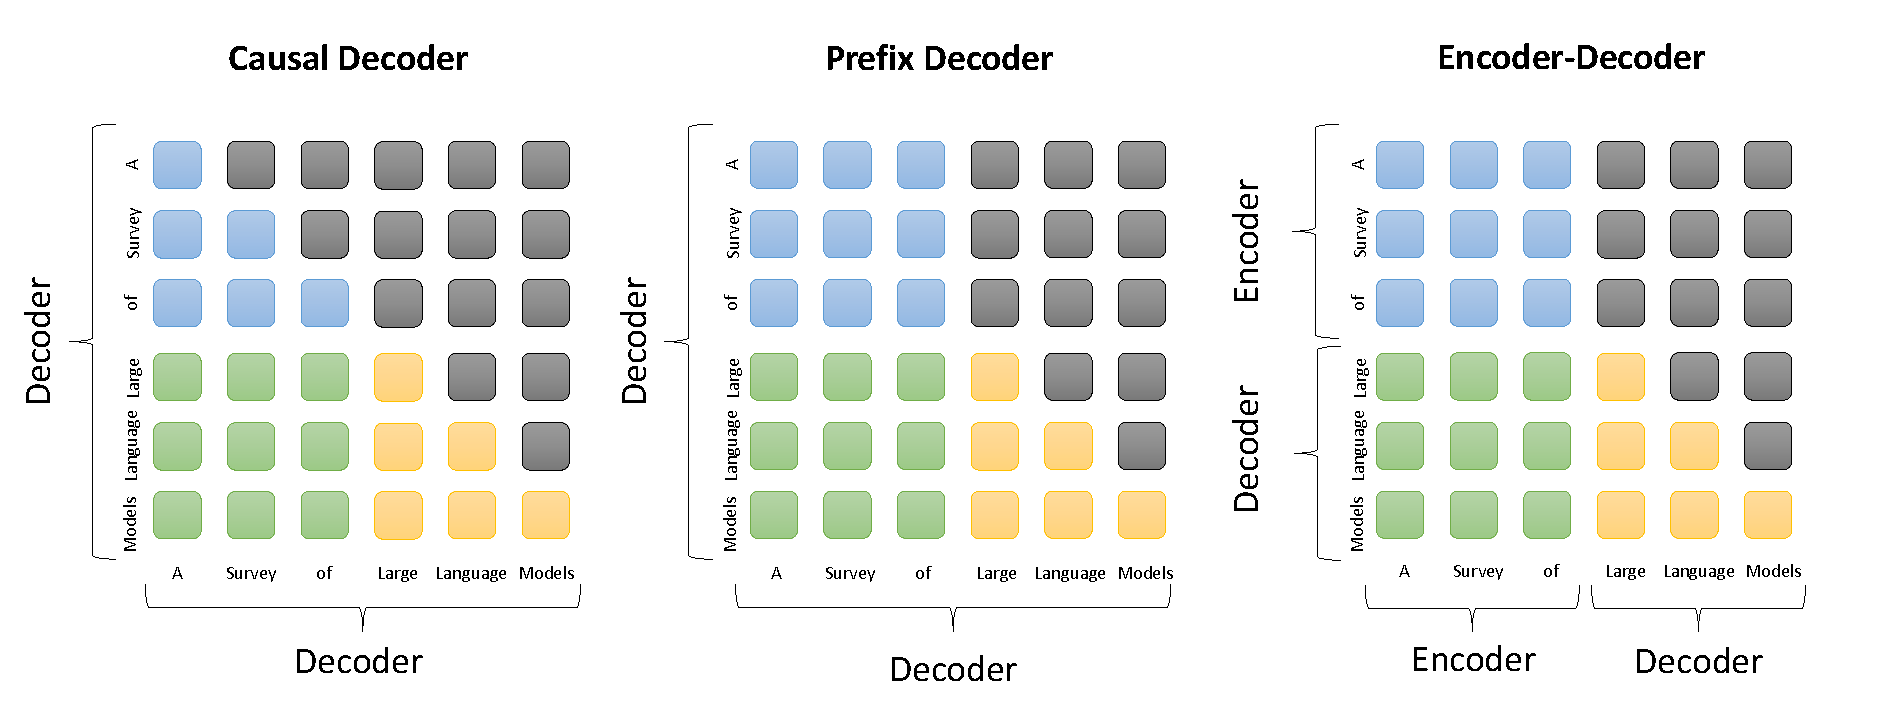
\includegraphics[width=\textwidth]{images/architectures.pdf}
    \caption{A comparison of the attention patterns in  three mainstream architectures. Here, the blue, green, yellow and grey rounded rectangles indicate the attention between prefix tokens, attention between prefix and target tokens, attention between target tokens, and masked attention respectively.}
    \label{fig:architectures}
\end{figure*}


Due to the excellent parallelizability and capacity, the Transformer architecture~\cite{Vaswani-NIPS-2017-Attention} has become the de facto backbone to develop various LLMs, making it possible to scale language models to hundreds or thousands of billions of parameters.    
In general, the mainstream architectures of existing LLMs can be roughly categorized into three major types, namely encoder-decoder, causal decoder, and prefix decoder, %
as shown in Figure~\ref{fig:architectures}. 

\paratitle{Encoder-decoder Architecture.}
The vanilla Transformer model is built on the encoder-decoder architecture~\cite{Vaswani-NIPS-2017-Attention}, which consists of two stacks of Transformer blocks as the encoder and decoder, respectively. 
The encoder adopts stacked multi-head self-attention layers to encode the input sequence for generating its latent representations, while the decoder performs cross-attention on these representations and autoregressively generates the target sequence. %
Encoder-decoder PLMs (\eg T5~\cite{Raffel-JMLR-2020-Exploring} and BART~\cite{Lewis-ACL-2020-BART}) have shown effectiveness on a variety of NLP tasks.
{
So far, there are only a small number of LLMs that are built based on the encoder-decoder architecture, \eg Flan-T5~\cite{Chung-arxiv-2022-Scaling}. We leave a detailed discussion about the architecture selection  in Section~\ref{sec-summary-arc}.  
}

\paratitle{Causal Decoder Architecture.} 
The causal decoder architecture incorporates the unidirectional attention mask, to guarantee that each input token can only attend to the past tokens and itself. 
The input and output tokens are processed in the same fashion through the decoder. As representative language models of this architecture, the GPT-series models~\cite{radford-openai-2018-improving,radford-blog-2019-language,Brown-NeurIPS-2020-Language} are developed based on the causal-decoder architecture. 
In particular, GPT-3~\cite{Brown-NeurIPS-2020-Language} has successfully demonstrated the effectiveness of this architecture, also showing an amazing in-context learning capability of LLMs.
Interestingly, GPT-1~\cite{radford-openai-2018-improving} and GPT-2~\cite{radford-blog-2019-language} do not exhibit such superior abilities as those in GPT-3, and it seems that scaling plays an important role in increasing the model capacity of this model architecture. 
So far, 
the causal decoders have been widely adopted as the architecture of LLMs by various existing LLMs, such as OPT~\cite{Zhang-arxiv-2022-OPT}, BLOOM~\cite{Scao-arxiv-2022-BLOOM}, and Gopher~\cite{Rae-arxiv-2021-Scaling}. 
{
Note that both the causal decoder and prefix decoder discussed next belong to decoder-only architectures. When  mentioning  ``{decoder-only architecture}'', it mainly refers to the causal decoder architecture in existing literature, unless specified. }

\paratitle{Prefix Decoder Architecture.} 
The prefix decoder architecture {(\aka non-causal decoder~\cite{Zhang-ICML-2022-Examining})}  revises the masking mechanism of causal decoders, to enable performing bidirectional attention over the prefix tokens~\cite{Dong-NIPS-2019-Unified} and unidirectional attention only on generated tokens. 
In this way, like the encoder-decoder architecture, the prefix decoders can bidirectionally encode the prefix sequence and autoregressively predict the output tokens one by one, where the same parameters are shared during encoding and decoding. 
Instead of pre-training from scratch, a practical suggestion is to continually train causal decoders and then convert them into prefix decoders for accelerating convergence~\cite{Wang-ICML-2022-What}, \eg U-PaLM~\cite{Tay-arxiv-2022-Transcending} is derived from PaLM~\cite{Chowdhery-arxiv-2022-PaLM}. Existing representative LLMs based on prefix decoders include GLM-130B~\cite{Zeng-arxiv-2022-GLM} and U-PaLM~\cite{Tay-arxiv-2022-Transcending}.

\paratitle{Mixture-of-Experts.} For the above three types of architectures, we can  further extend  them via  the mixture-of-experts (MoE) scaling, in which a subset of neural network weights for each input are sparsely activated, \eg Switch Transformer~\cite{Fedus-JMLR-2021-Switch} and GLaM~\cite{Du-ICML-2022-GLaM}.  %
{The major merit is that MoE is a flexible way to scale up the model parameter while maintaining a constant computational cost~\cite{Fedus-JMLR-2021-Switch}.} It has been shown that substantial  performance improvement can be observed by increasing either the number of experts or the total parameter size~\cite{Clark-ICML-2022-Unified}.  {Despite the merits, training large MoE models may suffer from instability issues due to the complex, hard-switching nature of the routing operation. 
To enhance the training stability of MoE-based language models, techniques such as selectively using high-precision tensors in the routing module or initializing the model with a smaller range have been introduced~\cite{Fedus-JMLR-2021-Switch}.
More recently, there is  widespread speculation that GPT-4 has been developed based on  the MoE architecture, but without official verification. 
} 

\paratitle{Emergent Architectures.} %
{The conventional Transformer architectures typically suffer from quadratic computational complexity. Because of this, efficiency  has become an important issue when training and making inference with long inputs. To improve efficiency, some studies aim to devise new architectures for language modeling, including parameterized state space models (\eg S4~\cite{gu-2022-iclr-efficiently}, GSS~\cite{Mehta-2022-arxiv-long}, and H3~\cite{dao-2022-arxiv-hungry}), long convolutions like Hyena~\cite{poli-2023-icml-hyena}, and Transformer-like architectures that incorporate recursive update mechanisms (\eg RWKV~\cite{peng-2023-arxiv-rwkv} and RetNet~\cite{sun-2023-arxiv-retnet}).  
{The key merits of these new architectures are twofold. First, these models can generate outputs recursively like RNNs, meaning that they only need to refer to the  single previous state during decoding. It makes the decoding process more efficient as it eliminates the need to revisit all previous states as in conventional Transformers. Second, these models have the capacity to encode an entire sentence in parallel like Transformers. This contrasts with conventional RNNs which has to encode sentences on a token-by-token basis. Thus, they can  benefit from the parallelism of GPUs with techniques such as Parallel Scan~\cite{smith-2023-iclr-s5,orvieto-2023-icml-lru}, FFT~\cite{poli-2023-icml-hyena,peng-2023-arxiv-rwkv}, and Chunkwise Recurrent~\cite{sun-2023-arxiv-retnet}. These techniques enable models with these new architectures to be trained in a highly parallel and efficient manner.}

\subsubsection{Detailed Configuration}
\label{sec:configuration}

\begin{table*}[htb]
    \centering
    
   \caption{Detailed formulations for the network configurations. Here, Sublayer denotes a FFN or a self-attention module in a Transformer layer, $d$ denotes the size of hidden states, $\mathbf{p}_i$ denotes position embedding at position $i$, $A_{ij}$ denotes the attention score between a query and a key, $r_{i-j}$ denotes a learnable scalar based on the offset between the query and the key, and $\mathbf{R}_{\Theta, t}$ denotes a rotary matrix with rotation degree $t\cdot\Theta$.}
    \begin{tabular}{c|c|l}
    \toprule
    \textbf{Configuration}& \textbf{Method }& \textbf{Equation}\\\midrule
    \multirow{3}{*}{Normalization position}     &Post Norm~\cite{Vaswani-NIPS-2017-Attention} & $\mathrm{Norm(}\mathbf{x} \mathrm{+ Sublayer(}\mathbf{x}\mathrm{))}$  \\
         &Pre Norm~\cite{radford-blog-2019-language} &$\mathbf{x}+\mathrm{Sublayer}(\mathrm{Norm}(\mathbf{x}))$ \\
         &Sandwich Norm~\cite{Ding-NIPS-2021-CogView} & $\mathbf{x}+\mathrm{Norm}(\mathrm{Sublayer}(\mathrm{Norm}(\mathbf{x})))$\\
         \midrule
         \multirow{3}{*}{Normalization method}& LayerNorm~\cite{Jimmy-arxiv-2016-Layer}&$ \frac{\mathbf {x} -\mathbf \mu}{\mathbf \sigma}\cdot \gamma +\beta, \text{~~~} \mathbf \mu=\frac 1 d \sum_{i=1}^d  x_i, \text{~~~} \mathbf \sigma=\sqrt{\frac 1 d \sum_{i=1}^d ( x_i-\mathbf \mu))^2}$         \\
         & RMSNorm~\cite{Zhang-NIPS-2019-Root}&  $ \frac {\mathbf x}{\mathrm{RMS}(\mathbf x)} \cdot \gamma, \text{~~~} \mathrm{RMS}(\mathbf x)=\sqrt {\frac 1 d \sum_{i=1}^d  x_i^2}$\\
         & DeepNorm~\cite{Wang-arxiv-2022-DeepNet}& $\mathrm {LayerNorm}(\alpha \cdot \mathbf x + \mathrm{Sublayer}(\mathbf x))$\\
         \midrule
    \multirow{5}{*}{Activation function}& ReLU~\cite{Vinod-ICML-2010-Rectified}& $\mathrm {ReLU}(\mathbf{x}) = \max(\mathbf{x},\mathbf{0})$\\
    & GeLU~\cite{Wang-EMNLP-2018-GLUE}&$\mathrm {GeLU}(\mathbf{x}) = \mathrm{0.5}\mathbf{x} \otimes [1+\mathrm{erf}(\mathbf{x}/\sqrt{2})], \text{~~~} \mathrm{erf}(x)=\frac 2 {\sqrt \pi}\int_0^x e^{-t^2} dt  $\\
    &Swish~\cite{Ramachandran-arXiv-2017-searching} & $\mathrm{Swish}(\mathbf{x}) = \mathbf x \otimes \mathrm{sigmoid}(\mathbf{x}) $\\
    & SwiGLU~\cite{Shazeer-arxiv-2020-GLU}&$\mathrm{SwiGLU}(\mathbf{x}_1,\mathbf{x}_2) = \mathrm{Swish}(\mathbf{x_1})\otimes \mathbf{x_2}$\\
    & GeGLU~\cite{Shazeer-arxiv-2020-GLU}& $\mathrm{GeGLU}(\mathbf{x}_1,\mathbf{x}_2) = \mathrm{GeLU}(\mathbf{x_1})\otimes \mathbf{x_2}$ \\
    \midrule
    \multirow{4}{*}{Position embedding}& Absolute~\cite{Vaswani-NIPS-2017-Attention}&$\mathbf x_i = \mathbf x_i + \mathbf p_i$ \\
    &Relative~\cite{Raffel-JMLR-2020-Exploring}& $A_{ij} = \mathbf W_q\mathbf x_i \mathbf x_j^T \mathbf W_k^T + r_{i-j}$\\
    &RoPE~\cite{Su-arxiv-2021-Roformer}& $A_{ij} = \mathbf W_q\mathbf x_i \mathbf R_{\Theta, i-j}\mathbf x_j^T\mathbf W_k^T =  (\mathbf W_q\mathbf x_i \mathbf R_{\Theta, i})(\mathbf W_k \mathbf x_j R_{\Theta,  j })^T$\\
    &ALiBi~\cite{Press-ICLR-2022-Train}& 
    $A_{ij} = \mathbf W_q \mathbf x_i \mathbf x_j^T\mathbf W_k^T - m (i-j)$\\  
    \bottomrule
    \end{tabular} 
    \label{tab:detailed_configuration}
\end{table*}

Since the launch of Transformer~\cite{Vaswani-NIPS-2017-Attention}, various improvements have been proposed to enhance its training stability, performance, and computational efficiency. In this part, we will discuss the corresponding 
configurations for 
four major parts of the Transformer, including normalization, position embeddings, activation functions, and attention and bias. 
To make this survey more self-contained, we present the detailed formulations for these configurations in Table~\ref{tab:detailed_configuration}. 

\paratitle{Normalization Methods.} {Training instability is a  challenging issue for pre-training  LLMs. To alleviate this issue, normalization is a widely adopted strategy to stabilize the training of neural networks. In the vanilla Transformer~\cite{Vaswani-NIPS-2017-Attention}, LayerNorm~\cite{Jimmy-arxiv-2016-Layer} is employed. Recently, several advanced normalization techniques have been proposed as alternatives to LayerNorm, \eg RMSNorm, and DeepNorm. }

{
    $\bullet$ \emph{LayerNorm.} In the early research, BatchNorm~\cite{Ioffe-2015-ICML-Batch} is a commonly used normalization method. However, it is difficult to deal with sequence data of variable lengths and small-batch data. Thus, LayerNorm~\cite{Jimmy-arxiv-2016-Layer} is introduced to conduct layerwise normalization.  Specifically, the mean and variance over all activations per layer are calculated to re-center and re-scale the activations. }

{
    $\bullet$ \emph{RMSNorm.} To improve the training speed of LayerNorm (LN), RMSNorm~\cite{Zhang-NIPS-2019-Root} is proposed by re-scaling the activations with only the root mean square (RMS) of the summed activations,  instead of the mean and variance. Related research has demonstrated its superiority in training speed and performance on Transformer~\cite{Narang-EMNLP-2021-Do}. Representative models that adopt RMSNorm include Gopher~\cite{Rae-arxiv-2021-Scaling} and Chinchilla~\cite{Hoffmann-arxiv-2022-Training}.}

{
    $\bullet$ \emph{DeepNorm.} DeepNorm is proposed by Microsoft~\cite{Wang-arxiv-2022-DeepNet} to stabilize the training of deep Transformers. 
    With DeepNorm as residual connections, Transformers can be scaled up to 1,000 layers~\cite{Wang-arxiv-2022-DeepNet}, which has shown  the advantages of stability and good performance. It has been adopted by GLM-130B~\cite{Zeng-arxiv-2022-GLM}.
    }
    
\paratitle{Normalization Position.} {In addition to the normalization method, normalization position also plays a  crucial role in the LLMs. There are generally three choices for the normalization position, \ie post-LN, pre-LN, and sandwich-LN. } 

{
    $\bullet$ \emph{Post-LN.} Post-LN is used in the vanilla  Transformer~\cite{Vaswani-NIPS-2017-Attention}, which is placed between residual blocks. However, existing work has found that the training of Transformers with post-LN tends  to be  instable due to the large gradients near the output layer~\cite{Xiong-ICML-2020-On}. Thus, post-LN is rarely employed in existing LLMs except combined with other strategies (\eg combining post-LN with pre-LN in GLM-130B~\cite{Zeng-arxiv-2022-GLM}).  }


{
    $\bullet$ \emph{Pre-LN.} Different from post-LN, pre-LN~\cite{Baevski-2019-ICLR-Adaptive} is applied before each sub-layer, and an additional LN is placed before the final prediction. Compared with post-LN, the Transformers with pre-LN are more stable in training. However, it performs worse than the variants with post-LN~\cite{liu-2020-EMNLP-Understanding}. Despite the decreasing performance, most LLMs still adopt pre-LN due to the training stability. } 
    {
    However, one exception is that pre-LN  has been found   unstable in GLM when training models more than 100B parameters~\cite{Zeng-arxiv-2022-GLM}.
    }


    $\bullet$ \emph{Sandwich-LN.} Based on pre-LN, Sandwich-LN~\cite{Ding-NIPS-2021-CogView} adds extra LN before the residual connections to avoid the  {value explosion issues in Transformer layer outputs.} However, it has been found that Sandwich-LN sometimes fails to stabilize the training of LLMs and may lead to the collapse of training~\cite{Zeng-arxiv-2022-GLM}.
    


 

\paratitle{Activation Functions.}
To obtain good performance, activation functions also need to be properly set in feed-forward networks. 
In existing LLMs, GeLU activations~\cite{Dan-arxiv-2016-Gaussian} are widely used. %
Specially, in the latest LLMs (\eg PaLM and LaMDA), variants of GLU activation~\cite{Dauphin-ICML-2017-Language,Shazeer-arxiv-2020-GLU} have also been utilized, especially the SwiGLU and GeGLU variants, which 
often achieve better performance in practice~\cite{Narang-EMNLP-2021-Do}. However, compared with GeLU, they require extra parameters (about 50\%) in the feed-forward networks~\cite{Le-EMNLP-2022-What}.

\paratitle{Position Embeddings.} 
Since the self-attention modules
in Transformer are permutation equivariant, position embeddings~(PE) are employed to inject absolute or relative position information for modeling sequences. 

{
    $\bullet$ \emph{Absolute position embedding.} In the vanilla Transformer~\cite{Vaswani-NIPS-2017-Attention}, absolute position embeddings are employed. At the bottoms of the encoder and the decoder, the absolute positional embeddings are added to the input embeddings. 
    There are two variants of absolute position embeddings proposed in the vanilla Transformer~\cite{Vaswani-NIPS-2017-Attention}, \ie sinusoidal and learned position embeddings, where the latter is commonly used in existing pre-trained language models. } %

    $\bullet$ \emph{Relative position embedding.} Unlike absolute position embeddings, relative positional embeddings are generated according to the offsets between keys and queries~\cite{shaw-2018-acl-self}.  %
    {A popular variant of relative PE was introduced in Transformer-XL~\cite{dai-2019-acl-transformer,Yang-NeurIPS-2019-xlnet}. The calculation of attention scores between keys and queries has been modified to introduce learnable embeddings corresponding to relative positions.}
 {T5~\cite{Raffel-JMLR-2020-Exploring} further simplified relative positional embeddings, which was subsequently adopted by Gopher~\cite{Rae-arxiv-2021-Scaling}.}
    Specifically, it adds learnable scalars to the attention scores, where the scalars are calculated based on the distances between the positions of the query and the key. Compared with the absolute PE, Transformers with relative position embedding can generalize to sequences longer than those sequences for training, \ie extrapolation~\cite{Press-ICLR-2022-Train}. 

    $\bullet$ \emph{Rotary Position Embedding.} 
{Rotary position embedding (RoPE)~\cite{Su-arxiv-2021-Roformer} 
    sets specific rotatory matrices based on the absolute position of each key or query.
    The scores between keys and queries can be computed with relative position information (Table~\ref{tab:detailed_configuration}).} 
    {RoPE combines each consecutive pair of elements in query and key vectors as \emph{a dimension},   so there are $d/2$  dimensions for an original $d$-length embedding. For each dimension $i \in \{1, \dots, d/2\}$, the  pair of involved elements will rotate based on the rotation angle $t\cdot \theta_i$, where $t$ denotes  the position index and $\theta_i$ is the basis in the dimension. Following sinusoidal position embeddings~\cite{Vaswani-NIPS-2017-Attention}, RoPE defines the \emph{basis}  $\theta_i$ as an exponentiation of the \emph{base} $b$ (set to $10000$ by  default):}
\begin{equation}
    \Theta = \{\theta_i = b^{-2(i-1)/d} | i \in \{1, 2, \dots , d/2 \}\}.\label{eq:basis}
\end{equation}
{Furthermore, a recent study~\cite{Peng-arxiv-2023-Yarn} defines the distance required to rotate one cycle ($2\pi$) for each dimension as wavelength:}
\begin{equation}
      \lambda_i = 2\pi b^{2(i-1)/d}=2 \pi / \theta_i.\label{eq:wavelength}
\end{equation}       
Due to the excellent performance and the long-term decay property, RoPE is widely adopted in the latest LLMs, \eg PaLM~\cite{Chowdhery-arxiv-2022-PaLM} and LLaMA~\cite{Touvron-arxiv-2023-LLaMA}. Based on RoPE,  xPos~\cite{Sun-2022-arxiv-Length} further improves the translation invariance and length extrapolation of Transformer. At each dimension of the rotation angle vector, xPos adds a special exponential decay that is smaller when the basis is larger. It can alleviate the unstable phenomenon {during training} as the distance increases. 
    

    $\bullet$ \emph{ALiBi.} ALiBi~\cite{Press-ICLR-2022-Train} is proposed to improve the extrapolation of Transformer. Similar to relative position embedding, it biases attention scores with a penalty based on the distances between keys and queries. 
    {Different from the relative positional embedding methods like T5~\cite{Raffel-JMLR-2020-Exploring}, the penalty scores in ALiBi are pre-defined without any trainable parameters.}
    Empirical results in~\cite{Press-ICLR-2022-Train} have shown that ALiBi has {a better extrapolation performance on sequences that are longer than those for training than several popular 
    position embedding methods such as  sinusoidal PE~\cite{Vaswani-NIPS-2017-Attention}, RoPE~\cite{Su-arxiv-2021-Roformer}, and T5 bias~\cite{Raffel-JMLR-2020-Exploring}. }
    In addition, it has been shown that ALiBi can also improve training stability in BLOOM~\cite{Scao-arxiv-2022-BLOOM}.



\paratitle{Attention.} 
Attention mechanism is a critical component of Transformer. It allows the tokens across the sequence to interact with each other and compute the representations of the input and output sequence. 

{
    $\bullet$ \emph{Full attention}. In the vanilla  Transformer~\cite{Vaswani-NIPS-2017-Attention}, the attention mechanism is conducted in a pairwise way, considering the relations between all token pairs in a sequence. It 
    adopts scaled dot-product attention, in which the hidden states are mapped into queries, keys, and values. 
    Additionally, Transformer uses multi-head attention instead of single attention, projecting the queries, keys, and values with different projections in different heads. The concatenation of the output of each head is taken as the final output.}

{
    $\bullet$ \emph{Sparse attention}. A crucial challenge of full attention is the quadratic computational complexity, which becomes a burden when dealing with long sequences. Therefore, various efficient Transformer variants are proposed to reduce the computational complexity of the attention mechanism~\cite{Peng-ICLR-2021-Random, Zaheer-NIPS-2020-Big}. For instance, locally banded sparse attention (\ie Factorized Attention~\cite{Child-arxiv-2019-Generating} has been adopted  in GPT-3~\cite{Brown-NeurIPS-2020-Language}. Instead of the whole sequence, each query can only attend to a subset of tokens based on the positions. }


    $\bullet$ \emph{Multi-query/grouped-query attention}. Multi-query attention refers to the attention variant
    where different heads share  {the same  linear transformation matrices on the keys and values~\cite{Shazeer-2019-arxiv-Fast}.} 
    It achieves higher inference speed {with only a minor sacrifice in model quality.}
    Representative models with multi-query attention include PaLM~\cite{Chowdhery-arxiv-2022-PaLM} and StarCoder~\cite{Li-2023-arxiv-Starcoder}.  %
    {To make a trade-off between multi-query attention and multi-head attention, grouped-query attention (GQA)~\cite{Ainslie-2023-arxiv-gqa} has been explored. In GQA, heads are assigned into different groups, and those heads that belong to the same group will share the same transformation matrices. Specially, GQA has been adopted and empirically tested in the recently released LLaMA 2 model~\cite{Touvron-2023-llama2-arxiv}.}

    $\bullet$ \emph{FlashAttention}. Different from most existing approximate attention methods that trade-off model quality to improve the computing efficiency, FlashAttention~\cite{Dao-NeurIPS-2020-FLASH} proposes to optimize the speed and memory consumption of attention modules on GPUs from an IO-aware perspective. There exist different levels of memory on modern GPUs, \eg SRAM with a fast IO and HBM with a relatively slow IO. FlashAttention organizes the input into blocks and introduces necessary recomputation, both to make better use of the fast memory SRAM.  Implemented as a fused kernel in CUDA, FlashAttention has been integrated into PyTorch~\cite{Paszke-NeurIPS-2019-Pytorch}, DeepSpeed~\cite{Rasley-KDD-2020-DeepSpeed}, and Megatron-LM~\cite{Shoeybi-arXiv-2019-Megatron}. {The updated version FlashAttention-2~\cite{Dao-2023-arxiv-flashattention2} further optimizes the work partitioning of GPU thread blocks and warps, leading to around 2$\times$ speedup when compared to the original FlashAttention.}

    $\bullet$ \emph{PagedAttention}.  %
    {It has been observed when LLM are deployed on servers, GPU memory is largely occupied by cached attention key and value tensors (called \emph{KV cache}). The major reason is that the input lengths are often varied, leading to fragmentation and over-reservation issues. Inspired by the classic paging technique in operating systems, PagedAttention has been proposed to improve the memory efficiency and throughput of deployed LLMs~\cite{vllm-pagedattention}. In detail, PagedAttention partitions each sequence into subsequences, and the corresponding KV caches of these subsequences are allocated into non-contiguous physical blocks. The paging technique increases the GPU utilization  and enables efficient memory sharing in parallel sampling.}


To put all these discussions together, we summarize the suggestions from existing literature for detailed configuration.  
For stronger generalization and training stability, it is suggested to choose the pre RMSNorm for layer normalization, and SwiGLU or GeGLU as the activation function. %
{In addition,  LN may not be used immediately after embedding layers, which is likely to incur  performance degradation.} As for position embeddings, {RoPE} or ALiBi is a better choice since it performs better on long sequences. %

\subsubsection{Pre-training Tasks}
Pre-training plays a key role that encodes general knowledge from large-scale corpus into the massive model parameters. 
For training LLMs, there are two commonly used pre-training tasks, namely language modeling and denoising autoencoding. %



\paratitle{Language Modeling.} 
The language modeling task (LM) is the most commonly used objective to pre-train decoder-only LLMs, \eg GPT3~\cite{Brown-NeurIPS-2020-Language} and PaLM~\cite{Chowdhery-arxiv-2022-PaLM}. Given a sequence of tokens $\mathbf{x}=\{x_1,\dots,x_n\}$, the LM task aims to autoregressively predict the target tokens  %
{$x_i$ based on the preceding tokens $x_{<i}$ in a sequence}. A general  training objective is to maximize the following likelihood: %
\begin{equation}
    \mathcal{L}_{LM}(\mathbf{x})=\sum_{i=1}^n \log P(x_i|\mathbf{x}_{<i}).\label{eq:lm}
\end{equation}

Since most language tasks can be cast as the prediction problem based on the input,  %
{these decoder-only} LLMs might be potentially advantageous to implicitly learn how to accomplish these tasks in a unified LM way. 
Some studies have also revealed that  %
{decoder-only} LLMs can be naturally transferred to certain tasks by autoregressively predicting the next tokens~\cite{radford-blog-2019-language,Brown-NeurIPS-2020-Language}, without fine-tuning.  
An important variant of LM is the \emph{prefix language modeling} task,  %
{which is designed for pre-training models with the prefix decoder architecture.
The tokens within a randomly selected prefix would not be used in computing the loss of prefix language modeling.} 
{
With the same amount of tokens seen during pre-training, prefix language modeling  performs slightly worse than language modeling, since fewer tokens in the sequence are involved for model pre-training~\cite{Wang-ICML-2022-What}.} %


\paratitle{Denoising Autoencoding.} 
{
In addition to conventional LM, the denoising autoencoding task (DAE) has also been widely used to pre-train language models~\cite{Lewis-ACL-2020-BART,Raffel-JMLR-2020-Exploring}.
The inputs $\mathbf{x}_{\backslash \Tilde{\mathbf{x}}}$ for DAE task are corrupted text with randomly replaced spans. Then, the language models are trained to recover the replaced tokens $\Tilde{\mathbf{x}}$. Formally, the training objective of DAE is  denoted as follows:}
\begin{equation}
    \mathcal{L}_{DAE}(\mathbf{x})= \log P(\Tilde{\mathbf{x}}|\mathbf{x}_{\backslash \Tilde{\mathbf{x}}}).\label{eq:dae}
\end{equation}

However, the DAE task seems to be more complicated in implementation than LM task. As a result, it has not been widely used to pre-train  large language models. 
Existing LLMs that take DAE as pre-training objectives include T5~\cite{Raffel-JMLR-2020-Exploring} and GLM-130B~\cite{Zeng-arxiv-2022-GLM}. These models are mainly trained to recover the replaced spans in an autoregressive way.

\paratitle{Mixture-of-Denoisers.} Mixture-of-Denoisers (MoD)~\cite{Tay-arxiv-2022-UL2}, also  known as  UL2 loss, was introduced as a unified objective for pre-training language models. MoD regards both LM and DAE objectives as different types of denoising tasks, namely  %
{S-denoiser (LM), R-denoiser (DAE, short span and low corruption), and X-denoiser (DAE, long span or high corruption).}
Among the three denoising tasks, S-denoiser is similar to the conventional LM objective (Equation~\eqref{eq:lm}), while R-denoiser and X-denoiser are similar to DAE objectives (Equation~\eqref{eq:dae}) but differ from each other in the lengths of spans and ratio of corrupted text.  
{For input sentences started with different special tokens (\ie \{\texttt{[R]}, \texttt{[S]}, \texttt{[X]}\}), the model will be optimized using the corresponding denoisers.} 
MoD has been  
applied in the latest PaLM 2 model~\cite{Anil-arxiv-2023-palm2}.


\begin{figure}
    \centering
    \begin{tabular}{lc|lc|lc}
    \multicolumn{6}{c}{I am sleepy. I start a pot of \_\_\_\_\_} \\
    \midrule[0.3pt]
    coffee & 0.661 & strong & 0.008 & soup & 0.005 \\
    water & 0.119 & black & 0.008 & \dots & \dots \\
    tea & 0.057 & hot & 0.007 & happy & 4.3e-6 \\
    rice & 0.017 & oat & 0.006 & Boh & 4.3e-6 \\
    chai & 0.012 & beans & 0.006 & \dots & \dots \\
    \end{tabular}
    \caption{The probability distribution over the vocabulary in descending order for the next token of the context ``\emph{I am sleepy. I start a pot of}''. For ease of discussion, this example is given in word units instead of subword units. }
    \label{fig:decoding-example}
\end{figure}



\subsubsection{Long Context Modeling}
\label{sec:long_context}
In real applications, there is an increasing demand for long context modeling capacities of LLMs,  such as PDF processing and story writing~\cite{Yuan-2022-IUI-Wordcraft}. Many closed-source LLMs provide professional support for long text processing. For instance, OpenAI releases GPT-4 Turbo  with a 128K context window, and Anthropic releases Claude 2.1 with a 200K  context window. To enhance the long context modeling abilities, there are generally two feasible directions, namely scaling position embeddings and adapting context window. Next, we introduce the two parts in detail.  









\paratitle{Scaling Position Embeddings.}{
Transformer-based LLMs can learn effective position embeddings within the maximum training length.  Thus, when adapting LLMs to language tasks beyond the maximum training length, it is necessary to scale to larger position indices. 
Some specific position embeddings have been shown to possess a certain degree of ability to generalize to text beyond the training length,  which is formally termed \textit{extrapolation capability}, including  T5 bias~\cite{Raffel-JMLR-2020-Exploring}, ALiBi~\cite{Press-ICLR-2022-Train}, xPos~\cite{Sun-2022-arxiv-Length} and even NoPE~\cite{kazemnejad-arxiv-2023-impact}. 
{However, as one of the mainstream position embedding methods, RoPE exhibits limited extrapolation ability in empirical studies~\cite{Chen-arxiv-2023-Extending}.}  
In the following, we discuss several methods that can scale RoPE to longer texts.
}

{
$\bullet$~\emph{Direct model fine-tuning.} 
To adapt LLMs to a long context window, a straightforward approach is to directly fine-tune the models on long texts with the desired length. 
The context extension can be scheduled with increased lengths in a multi-stage approach (\eg 2K $\rightarrow$ 8K $\rightarrow$ 32K). 
To conduct effective extension, it needs specially prepared long texts for training. 
Specially, some recent study has shown that the quality is more important than the lengths of training text in long context models~\cite{xiong-arxiv-2023-effective}. However, a recent study has highlighted that
the fine-tuning approach tends to be inherently slow when adapting LLMs for long texts~\cite{Chen-arxiv-2023-Extending}.
}


$\bullet$~\emph{Position interpolation.} This method downscales the position indices within the original context window, to avoid out-of-distribution rotation angles during  pre-training~\cite{Chen-arxiv-2023-Extending, kaiokendev-github-2023-Things}. To be more specific, this approach multiplies all position indices by a coefficient $L/L'$ ($L < L'$), where $L$ and $L'$ represent the original and target context window length, respectively. {
Experimental results~\cite{Chen-arxiv-2023-Extending} have shown that this method can extend the context window effectively and efficiently},  compared to the above approach of direct model fine-tuning. However, it is worth noting that this technique may have an adverse impact on the model's performance when handling shorter texts\cite{Chen-arxiv-2023-Extending,Dong-arxiv-2023-BAMBOO}.}





$\bullet$~\emph{Position truncation.} To mitigate the challenges posed by out-of-distribution rotation angles, another practical approach is to truncate longer relative positions to satisfy the requirement of the maximum training length. Specifically, ReRoPE and LeakyReRoPE~\cite{su-online-2023-Rerope} introduce a pre-defined window length, which is smaller than the maximum training length. 
Position indices within this pre-defined window are retained, while those indices beyond the window are either truncated to the pre-defined window length or interpolated to align with the maximum training length. This strategy can reserve local position relationships and enhance the extrapolation capacity. %
{However, this approach needs to compute the attention matrices twice, accommodating additional computational budget.}



{
$\bullet$ \emph{Base modification.} 
LLMs are usually trained with a pre-set maximum training length, \eg 4096 in Llama 2~\cite{Touvron-2023-llama2-arxiv}. However, wavelengths in certain dimensions of RoPE may exceed the training length for longer text~\cite{Peng-arxiv-2023-Yarn}, so that language models have not undergone sufficient  training (\ie a complete rotation cycle) on these dimensions. Thus, when we adapt LLMs to longer texts, the rotation angles  for certain dimensions would be never seen in the training phase~\cite{Liu-arxiv-2023_scaling}. 
Given a fixed rotation angle $t\cdot \theta_i$,  a smaller basis $\theta_i$ allows for a greater distance $t$, \ie enabling the modeling of longer texts~\cite{Peng-arxiv-2023-Yarn, Roziere-arxiv-2023-codellama,xiong-arxiv-2023-effective}.
According to the formula $\theta_i=b^{-2(i-1)/d}$ in Equation~\ref{eq:basis}, decreasing the basis can be achieved by increasing the value of the base. In addition,
decreasing the base can also help re-scale the wavelengths of all dimensions below the training length, while it often needs continual pre-training to adapt the LLMs to long context windows~\cite{Liu-arxiv-2023_scaling}.
A recent study~\cite{Liu-arxiv-2023_scaling} has empirically compared these two base modification methods, and shown that decreasing the base demonstrates a better extrapolation capacity beyond the training length, while increasing the base performs better within the training length.
}







$\bullet$ \emph{Basis truncation.} Similar to the base modification, the truncation of the basis also concentrates on dealing with the singular dimensions with wavelengths exceeding the training length~\cite{Pal-arxiv-2023-giraffe}. According to the definition $\lambda_i=2\pi/\theta_i$ in Equation~\ref{eq:wavelength}, the dimension with a large wavelength $\lambda_i$ has a small basis $\theta_i$ accordingly. Based on this observation, this approach first defines a basis range $[a, c]$. 
{
Given the basis range, the value of basis is modified according to the following ways: (1) when $\theta_i\geq  c$, the value is retained, (2) when $\theta_i \leq a$, the value is set to zero, and (3) when $a < \theta_i < c$, the value is truncated to a fixed small value.} 
{Via basis truncation, the out-of-distribution rotation angles can be avoided at larger position indices. However, this approach does not perform very well at long context tasks~\cite{Pal-arxiv-2023-giraffe}.}


\paratitle{Adapting Context Window.}
{Since Transformer-based LLMs have limited context windows, they can not directly integrate or utilize the entire information of the  long sequences exceeding the context  window. To alleviate the limitation, several methods adapting LLMs to long context have been proposed, as discussed below.
}


{
$\bullet$ \emph{Parallel context window.} Inspired by fusion-in-decoder~\cite{Izacard-EACL-2021-Leveraging}, parallel context window methods~\cite{Partner-ACL-2023-Parallel,Hao-2022-arxiv-Structured} adopt a divide-and-conquer strategy to process input text. Specially, it divides the input text into multiple segments, each independently encoded with shared position embeddings. In the generation stage, the attention masks are modified to make that subsequent tokens can access to previous tokens in each segment.
Nevertheless, this method cannot distinguish the order of different segments, constraining the model capacity on certain tasks.}

{
$\bullet$ \emph{$\Lambda$-shaped context window.} 
Some prior work has revealed that LLMs tend to allocate greater attention weights to the starting and nearest tokens among all previous tokens~\cite{Beltagy-arxiv-2020-longformer,Xiao-arxiv-2023-Efficient}, so called the ``\emph{lost in the middle}'' phenomenon~\cite{Liu-arxiv-2023-Lost}.}
Based on this observation, 
LM-Infinite~\cite{Han-arxiv-2023-LMinfinite} and StreamingLLM~\cite{Xiao-arxiv-2023-Efficient} propose to employ a ``$\Lambda$-shaped'' attention mask, which selectively preserves the initial tokens and the nearest tokens that each query can attend to and then discards any tokens beyond this scope.  %
{Experiments demonstrate that this method can facilitate extra-long text generation with a fixed memory~\cite{Xiao-arxiv-2023-Efficient}.}  However, it may struggle to model the long-range dependency in prompts, {since it cannot effectively utilize the information from the discarded tokens~\cite{Xiao-arxiv-2023-Efficient}.}

{
$\bullet$ \emph{External memory.}
It has been shown that a relatively small subset of tokens can effectively capture the majority of attention patterns in a Transformer~\cite{Bertsch-arxiv-2023-Unlimiformer}, \ie the top-$k$ attention keys can well approximate the original full attention. Therefore, a number of studies propose to store the past keys in external memory and utilize a $k$-NN search method to retrieve the $k$ most relevant  tokens for generation~\cite{Wu-ICLR-2022-Memorizing, Bertsch-arxiv-2023-Unlimiformer, Tworkowski-arxiv-2023-Focused}. For a decoder model, 
it typically employs one certain layer to access these top-$k$ external tokens, while still adopts the normal context window in the rest layers~\cite{Wu-ICLR-2022-Memorizing,Tworkowski-arxiv-2023-Focused}.}

}











{In addition to the studies based on vanilla Transformer, there are a surge of Transformer variants with efficient attentions and other efficient architectures, aiming to alleviate high computational cost for modeling long texts. These studies have been extensively discussed in Section~\ref{sec:archs} and Section~\ref{sec:configuration}. 
{Furthermore,  context compression and prompting techniques (\eg iterative reasoning~\cite{Chen-arxiv-2023-Walking}) have also been proven to be a viable strategy for  handling long text tasks}~\cite{zhou-arxiv-2023-recurrentgpt,Packer-arxiv-2023-MemGPT,Chen-arxiv-2023-Walking,Xu-arxiv-2023-retrieval}, without the need of model adaption.}

\subsubsection{Decoding Strategy}
\label{sec-decoding}
After the LLMs have been pre-trained, it is essential to employ a specific decoding strategy to generate the appropriate output from the LLMs. 

\paratitle{Background.} We start the discussion with the prevalent decoder-only architecture, and introduce the auto-regressive decoding mechanism.  Since such LLMs are pre-trained based on the  language modeling task (Equation~\ref{eq:lm}), a basic decoding method is \emph{greedy search} that predicts the most likely token at each step based on the previously generated tokens, formally modeled as:
\begin{equation}
{ x_i = \underset{x}{\arg\max} P(x |\mathbf{x}_{<i}),}
\end{equation}
where $x_i$ is the token with the highest probability at $i$-th step of generation conditioned on the context $\mathbf{x}_{<i}$. For instance in Figure~\ref{fig:decoding-example}, when predicting the next token of the sentence \emph{``I am sleepy. I start a pot of''}, greedy search selects the token ``coffee'' which has the highest probability at the current step. Greedy search can achieve satisfactory results in  text generation tasks (\eg machine translation and text summarization), in which  the output is highly dependent on the input~\cite{Murray-WMT-2018-Correcting}. However, in terms of open-ended generation tasks (\eg story generation and dialog), greedy search sometimes tends to generate awkward and repetitive sentences~\cite{Holtzman-2020-ICLR-The}.


As another alternative decoding strategy, sampling-based methods are proposed to randomly select the next token based on the probability distribution to enhance the randomness and diversity during generation:
\begin{equation}
    x_i \sim P(x|\mathbf{x}_{<i}).
\end{equation} 
For the example in  Figure~\ref{fig:decoding-example}, sampling-based methods will sample the word ``coffee'' with higher probability while also retaining the possibilities of selecting the rest words, ``water'', ``tea'', ``rice'', \etc.



Not limited to the decoder-only architecture, these two decoding methods can be generally applied to encoder-decoder models and prefix decoder models in a similar way.   


\paratitle{Improvement for Greedy Search.}
Selecting the token with the highest probability at each step may result in overlooking a sentence with a higher overall probability but a lower local estimation. Next, we introduce several improvement strategies  to alleviate this issue.

$\bullet$ \emph{Beam search.} 
Beam search~\cite{CMU-book-1977-speech} retains the sentences with the $n$ (beam size) highest probabilities at each step during the decoding process, and finally selects the generated response with the top probability. Typically, the beam size is configured within the range of 3 to 6. However, opting for a larger beam size might result in a decline in performance~\cite{Koehn-ACL-2017-Six}.


$\bullet$ \emph{Length penalty.} 
Since beam search favours shorter sentences, imposing length penalty (\aka length normalization) is a commonly used technique~\cite{Wu-arxiv-2016-Google} to overcome this issue, which normalizes the sentence probability according to the sentence length (divided by an exponential power $\alpha$ of the length).

Besides, some researchers~\cite{Paulus-iclr-2018-A} propose to penalize the generation of previously  generated tokens or $n$-grams to alleviate the issue of repetitive generation. In addition, diverse beam search~\cite{Vijayakumar-arxiv-2016-Diverse} can be leveraged to produce a set of diverse outputs based on the same input.

\paratitle{Improvement for Random Sampling.}
Sampling-based methods sample the token over the whole vocabulary, which may select wrong or irrelevant tokens (\eg ``happy'' and ``Boh'' in Figure~\ref{fig:decoding-example}) based on the context. To improve the generation quality, several strategies have been proposed for mitigating or preventing  the selection of words with exceedingly low probabilities.

$\bullet$ \emph{Temperature sampling.}
To modulate the randomness of sampling, a practical method is to adjust the temperature coefficient of the softmax function for computing the probability of the $j$-th token over the vocabulary:
\begin{equation}
    P(x_j|\mathbf{x}_{<i}) = \frac{\exp{(l_j/t)}}{\sum_{j'} \exp{(l_{j'}/t)}},
\end{equation}
where $l_{j'}$ is the logits of each word and $t$ is the temperature coefficient.  Reducing the temperature $t$ increases the chance of selecting words with high probabilities while decreases the chances of selecting words with low probabilities. 
When $t$ is set to 1, it becomes the default random sampling; when $t$ is approaching 0, it is equivalent to greedy search. 
In addition, when $t$ goes to infinity, it degenerates to uniform sampling. 

$\bullet$ \emph{Top-$k$ sampling.} 
Different from temperature sampling, top-$k$ sampling directly truncates the tokens with lower probability and only samples from the tokens with the top $k$ highest probabilities~\cite{Fan-2018-ACL-Hierarchical}. For example in Figure~\ref{fig:decoding-example}, top-$5$ sampling will sample from the words ``coffee'', ``water'', ``tea'', ``rice'', and ``chai'' from their re-scaled probabilities.

$\bullet$ \emph{Top-$p$ sampling.} 
Since top-$k$ sampling does not consider the overall  possibility distribution, a constant value of  $k$  may be not be suitable for different contexts. Therefore, top-$p$ sampling (\aka nucleus sampling) is proposed by sampling from the smallest set having a cumulative probability above (or equal to) $p$~\cite{Holtzman-2020-ICLR-The}. In practice, the smallest set can be constructed by gradually adding tokens from the vocabulary sorted in descending order of generative probability, until their cumulative value exceeds $p$.

Recently, researchers have also explored other sampling strategies for LLMs. For instance, \emph{$\eta$-sampling}~\cite{Hewitt-emnlp-2022-Truncation} further improves top-$p$ sampling by introducing a dynamic threshold based on the probability distribution. Furthermore, \emph{contrastive search}~\cite{Su-2022-NIPS-A} and \emph{typical sampling}~\cite{Meister-TACL-2023-Locally} can be utilized to improve the generation coherence during decoding. 
{Since it has been found that large models tend to assign higher probability to important tokens compared to small models, \emph{contrastive decoding}~\cite{Li-ACL-2023-Contrastive} utilizes a larger LM (\eg OPT-13B) and a smaller LM (\eg OPT-125M) to measure their log-likelihood differences. Subsequently, tokens are sampled based on the delta value of the probability distribution, thereby amplifying the impact of important tokens.} 
{Based on this contrastive idea, DoLa~\cite{Chuang-arxiv-2023-DoLa} further extends this approach to contrasting the logits across different layers of a single LLM, as higher layers tend to assign more weight to important tokens.}









\begin{center}
\begin{tcolorbox}[colback=blue!5!white,colframe=blue!55!black,width=0.48\textwidth,title={Memory Wall}]
{{When generating a new token, the most time-consuming steps  revolve around data transfer and weight computation. A main issue is the significant amount of time overwhelmed by data transfer, often referred to as the \emph{memory wall} issue.} 

\vspace{0.5em}

{To  address this issue, researchers formally quantify data transfer from GPU memory to GPU caches using the number of bytes in I/O, and they assess weight computation by measuring the number of FLOPs~\cite{Chen-blog-2023-Dissecting}. Specifically, let $b$, $s$, $n$, $d$, and $h$ denote the batch size, sequence length, number of attention heads, hidden size of each head, and overall hidden size ($h = n \cdot d$), respectively. During the layer-wise multi-head self-attention calculation in causal decoder, the I/O bytes and FLOPs at each decoding step can be expressed as $8bsn + 4bsnd + 4bnd$ and $8bsnd$, respectively~\cite{Chen-blog-2023-Dissecting}.}

\vspace{0.5em}


{\emph{Arithmetic intensity} is further defined as the ratio of FLOPs to I/O bytes:}

\begin{equation}
    \text{intensity} = \frac{\text{FLOPs}}{\text{I/O bytes}}=\frac{2}{1 + \frac{2}{d} + \frac{1}{s}}
\end{equation}

{Let's consider LLaMA 13B ($d = 128$) with a sequence length of 1024 ($s=1024$) as an  example. The calculated arithmetic intensity is $1.97$. However, the A100 80G GPU can perform $312$ TFLOPs and transfer $2$ TB of data in one second, \ie its ideal arithmetic intensity is $156$. This indicates that the bottleneck in attention calculation lies in the process of data transfer (\ie excessive I/O loading).}



}
\end{tcolorbox}
\end{center}


\paratitle{Decoding Efficiency Issues.}
In this part, we briefly analyze the decoding efficiency issues of LLMs. 
{Overall, the decoding process of LLMs can be divided into two stages for overhead analysis:  (1) the \emph{prefill} stage, which computes the hidden states of the input sequence, and (2) the \emph{incremental decoding} stage, which generates a token and updates hidden states in an auto-regressive manner~\cite{Sheng-ICML-2023-FlexGen}. As shown in the above \emph{memory wall} box, the arithmetic intensity of the incremental decoding stage is only $1.97$, which is far from the expected value of 156 (calculated according to the standard configuration of A100 80GB GPU). In contrast, the arithmetic intensity of the prefill stage achieves $113.78$ for LLaMA-13B. Consequently, existing work mainly investigates how to enhance the efficiency of the incremental decoding algorithm, which can be categorized into two main approaches:}


{$\bullet$ \emph{Reducing data transfer} mainly focuses on optimizing GPU memory access, thereby increasing the arithmetic intensity. As introduced in Section~\ref{sec:configuration}, KV cache can avoid redundant computation of previous tokens and PagedAttention   allocates KV caches into continuous blocks to reduce memory fragmentation. Furthermore, Flash-Decoding~\cite{Dao-stanford-2023-Flash} speeds up attention computation by loading the keys and values in parallel, especially effective for long text generation. As another alternative approach, multi-query and grouped-query attention can reduce the GPU memory bandwidth overhead by sharing KV parameters (loading fewer weights).}

{$\bullet$ \emph{Decoding strategy optimization} aims to improve the sequential nature of the auto-regressive generation manner in different ways. As a representative study, \emph{speculative decoding}~\cite{Yaniv-ICML-2023-Fast,Chen-arxiv-2023-Accelerating} first leverages a compact but efficient model (\eg a $n$-gram model or a small PLM) to generate short segments and then utilizes the LLM to verify and correct these drafts. It can lead to a notable {2$\times$ to 3$\times$ speedup} without  compromising the generation quality.
{Researchers further suggest several variants to improve the efficiency of this approach, such as a learning-based method to combine several small models~\cite{Miao-arxiv-2023-SpecInfer} and a stage-wise acceleration which employs a more smaller LM to accelerate the small LM first~\cite{Spector-2023-arxiv-Accelerating}.
In addition, token-level early-exit techniques have been proposed enabling the generation of a token at lower Transformer layers, rather than passing through all the layers~\cite{Corro-arxiv-2023-SkipDecode}. It can attain greater speedup, but at the cost of sacrificing generation quality.}












\paratitle{Practical Settings.} 
In practice, existing libraries (\eg Transformers~\cite{Wolf-EMNLP-2020-Transformers}) and public APIs of LLMs (\eg OpenAI) have supported various decoding strategies to serve different scenarios of text generation. Next, we present the decoding settings of several representative LLMs: 

$\bullet$ \emph{T5}~\cite{Raffel-JMLR-2020-Exploring} utilizes greedy search as the default setting and applies beam search (beam size of 4) with a length penalty {of 0.6} for translation and summarization tasks.

$\bullet$ \emph{GPT-3}~\cite{Brown-NeurIPS-2020-Language} employs beam search with a beam size of 4 and a length penalty of 0.6 for all generation tasks.

$\bullet$ \emph{Alpaca}~\cite{Taori-github-2023-Stanford} utilizes sampling-based strategies %
{with top-$k$ ($k=50$), top-$p$  ($p=0.9$)}, and temperature of 0.7 for open-ended generation.

$\bullet$ \emph{LLaMA}~\cite{Touvron-arxiv-2023-LLaMA} applies diverse decoding strategies tailored to specific tasks. For instance, it employs the greedy search for question answering tasks while utilizes a sampling strategy with the temperature settings of 0.1 (pass@1) and 0.8 (pass@100) for code generation.


$\bullet$ \emph{OpenAI API}  %
{supports several basic decoding strategies, including greedy search (by setting \texttt{temperature} to 0), beam search (with the setting \texttt{best\_of}), temperature sampling (with the setting \texttt{temperature}), nucleus sampling (with the setting \texttt{top\_p}). It also introduce parameters \texttt{presence\_penalty} and \texttt{frequency\_penalty} to control the repetition degree of generation.} 
{According to the OpenAI's document, their APIs would produce different outputs even if the input and the hyper-parameters are the same. Setting temperature to 0 can yield more deterministic outputs, albeit with a slight chance of variability.}


\subsubsection{Summary and Discussion}\label{sec-summary-arc}

The choice of architecture and pre-training tasks may incur different inductive biases for LLMs, which would lead to different model capacities. %
In this part, we discuss one open issue about the  architecture choice for LLMs.


\begin{center}
\begin{tcolorbox}[colback=blue!5!white,colframe=blue!55!black,width=0.48\textwidth,title={Why does Predicting the Next Word Works?}]
{
The essence of decoder-only architecture is to \emph{accurately predict the next word} for reconstructing the pre-training data. Till now, there has been no formal study that theoretically  demonstrates its advantage over other architectures. An interesting explanation was from  Ilya Sutskever during the interview held by Jensen Huang\footnote{https://www.nvidia.com/en-us/on-demand/session/gtcspring23-S52092/}. 
The original transcript from the interview was copied below\footnote{https://lifearchitect.ai/ilya/}:  
\\

\texttt{Say you read a detective novel. It’s like complicated plot, a storyline, different characters, lots of events, mysteries like clues, it’s unclear. Then, let’s say that at the last page of the book, the detective has gathered all the clues, gathered all the people and saying, "okay, I’m going to reveal the identity of whoever committed the crime and that person’s name is". Predict that word. ...\\
Now, there are many different words. But predicting those words better and better, the understanding of the text keeps on increasing. GPT-4 predicts the next word better. 
}
}
\end{tcolorbox}
\end{center}

\paratitle{Architecture Choice}.  {In earlier literature of pre-trained language models, there are lots of discussions on the effects of different architectures~\cite{Wang-ICML-2022-What,Tay-arxiv-2022-UL2}}.
However, most LLMs are developed based on the causal decoder architecture, and there  still lacks a theoretical analysis on its advantage over the other alternatives.  Next, we briefly summarize existing  discussions on this issue. 

$\bullet$ By pre-training with the LM objective, it seems that causal decoder architecture can achieve a superior zero-shot and few-shot generalization capacity. Existing research has shown that without multi-task fine-tuning, the causal decoder has better zero-shot performance than other architectures~\cite{Wang-ICML-2022-What}. The success of GPT-3~\cite{Brown-NeurIPS-2020-Language} has demonstrates that the large causal decoder model can be a good few-shot learner. In addition, instruction tuning and alignment tuning discussed in Section~\ref{sec-adaptation} have been proven to further enhance the capability of large causal decoder models~\cite{Wei-ICLR-2022-Finetuned,Ouyang-arxiv-2022-Training,Chung-arxiv-2022-Scaling}. 
    
$\bullet$  Scaling law has been widely observed in causal decoders. By scaling the model size, the dataset size, and the total computation, the performance of causal decoders can be substantially   improved~\cite{Kaplan-arxiv-2020-Scaling,Brown-NeurIPS-2020-Language}.
Thus, it has become an important strategy to increase the model capacity of the causal decoder via  scaling.  %
However, more detailed investigation on encoder-decoder models is still lacking, and more efforts are needed to investigate the performance of  encoder-decoder models at a large scale.
    
    

More research efforts about the discussions on architectures and pre-training objectives are in need to analyze how the choices of the architecture and pre-training tasks affect the capacity of LLMs, especially for encoder-decoder architectures.  
Despite the effectiveness of decoder-only architecture, it is also suggested to make more diverse exploration on architecture design. 
Besides the major architecture, the detailed configuration of LLM is also worth attention, which has been discussed in Section~\ref{sec:configuration}. 








\begin{table*}[htb]
    \centering
    \caption{Detailed optimization settings of several existing  LLMs. 
    }
\resizebox{2.05\columnwidth}{!}{
\begin{tabular}{lrrccccccc}
\toprule
\textbf{Model}          & \begin{tabular}[r]{@{}r@{}}\textbf{Batch Size}\\ \textbf{(\#tokens)}\end{tabular} & \begin{tabular}[r]{@{}r@{}}\textbf{Learning}\\ \textbf{Rate}\end{tabular}   & \textbf{Warmup} & \textbf{Decay Method}   & \textbf{Optimizer}                              & \begin{tabular}[l]{@{}l@{}}\textbf{Precision}\\ \textbf{Type}\end{tabular} & \begin{tabular}[l]{@{}l@{}}\textbf{Weight}\\ \textbf{Decay}\end{tabular}                & \begin{tabular}[l]{@{}l@{}}\textbf{Grad}\\ \textbf{Clip}\end{tabular} & \textbf{Dropout} \\ \midrule
GPT3~(175B)             & 32K→3.2M                                                                          & $6 \times 10^{-5}$                                                          & yes             & cosine decay to 10\%    & Adam                                            & FP16                                                                       & 0.1                                                                                     & 1.0                                                                   & -                \\
PanGu-$\alpha$~(200B)   & -                                                                                 & $2 \times 10^{-5}$                                                          & -               & -                       & Adam                                            & -                                                                          & 0.1                                                                                     & -                                                                     & -                \\
OPT~(175B)              & 2M                                                                                & $1.2 \times 10^{-4}$                                                        & yes             & manual decay            & AdamW                                           & FP16                                                                       & 0.1                                                                                     & -                                                                     & 0.1              \\
PaLM~(540B)             & 1M→4M                                                                             & $1 \times 10^{-2}$                                                          & no              & inverse square root     & Adafactor                                       & BF16                                                                       & $lr^2$                                                                                  & 1.0                                                                   & 0.1              \\
BLOOM~(176B)            & 4M                                                                                & $6 \times 10^{-5}$                                                          & yes             & cosine decay to 10\%    & Adam                                            & BF16                                                                       & 0.1                                                                                     & 1.0                                                                   & 0.0              \\
MT-NLG~(530B)           & 64 K→3.75M                                                                        & $5 \times 10^{-5}$                                                          & yes             & cosine decay to 10\%    & Adam                                            & BF16                                                                       & 0.1                                                                                     & 1.0                                                                   & -                \\
Gopher~(280B)           & 3M→6M                                                                             & $4 \times 10^{-5}$                                                          & yes             & cosine decay to 10\%    & Adam                                            & BF16                                                                       & -                                                                                       & 1.0                                                                   & -                \\
Chinchilla~(70B)        & 1.5M→3M                                                                           & $1 \times 10^{-4}$                                                          & yes             & cosine decay to 10\%    & AdamW                                           & BF16                                                                       & -                                                                                       & -                                                                     & -                \\
Galactica~(120B)        & 2M                                                                                & $7 \times 10^{-6}$                                                          & yes             & linear decay to 10\%    & AdamW                                           & -                                                                          & 0.1                                                                                     & 1.0                                                                   & 0.1              \\
LaMDA~(137B)            & 256K                                                                              & -                                                                           & -               & -                       & -                                               & BF16                                                                       & -                                                                                       & -                                                                     & -                \\
Jurassic-1~(178B)       & 32 K→3.2M                                                                         & $6 \times 10^{-5}$                                                          & yes             & -                       & -                                               & -                                                                          & -                                                                                       & -                                                                     & -                \\
LLaMA~(65B)             & 4M                                                                                & $1.5 \times 10^{-4}$                                                        & yes             & cosine decay to 10\%    & AdamW                                           & -                                                                          & 0.1                                                                                     & 1.0                                                                   & -                \\
LLaMA 2~(70B) & 4M & $1.5 \times 10^{-4}$ & yes & cosine decay to 10\% & AdamW & - & 0.1 & 1.0 & - \\
Falcon~(40B) & 2M & $1.85 \times 10^{-4}$ & yes & cosine decay to 10\% & AdamW & BF16 & 0.1 & - & - \\
GLM~(130B)              & 0.4M→8.25M                                                                        & $8 \times 10^{-5}$                                                          & yes             & cosine decay to 10\%    & AdamW                                           & FP16                                                                       & 0.1                                                                                     & 1.0                                                                   & 0.1              \\
T5~(11B)                & 64K                                                                               & $1 \times 10^{-2}$                                                          & no              & inverse square root     & AdaFactor                                       & -                                                                          & -                                                                                       & -                                                                     & 0.1              \\
ERNIE 3.0 Titan~(260B)  & -                                                                                 & $1 \times 10^{-4}$                                                          & -               & -                       & Adam                                            & FP16                                                                       & 0.1                                                                                     & 1.0                                                                   & -                \\
PanGu-$\Sigma$~(1.085T) & 0.5M                                                                              & $2 \times 10^{-5}$                                                          & yes             & -                       & Adam                                            & FP16                                                                       & -                                                                                       & -                                                                     & -                \\
\bottomrule\end{tabular}
}
\end{table*}

\subsection{Model Training}
\label{sec:training_settings}
In this part, we review the important settings, techniques, or tricks for training LLMs. 

\subsubsection{Optimization Setting}
 For parameter optimization of LLMs, we present the commonly used settings for batch training, learning rate, optimizer, and training stability.

\paratitle{Batch Training.}
For language model pre-training, existing work generally sets the batch size to a large number (\eg 2,048 examples or 4M tokens) to improve the training stability and {throughput}.
For LLMs such as GPT-3 and PaLM, they have introduced  a new strategy that dynamically increases the batch size during training, ultimately reaching a million scale. 
Specifically, the batch size of GPT-3 is gradually increasing from 32K to 3.2M tokens.
Empirical results have demonstrated that the dynamic  schedule of batch size can effectively stabilize the training process of LLMs~\cite{Chowdhery-arxiv-2022-PaLM}.

\paratitle{Learning Rate.}
Existing LLMs usually adopt a similar learning rate schedule with the warm-up and decay strategies during pre-training.
Specifically, in the initial 0.1\% to 0.5\% of the training steps, a linear warm-up schedule is employed for gradually increasing the learning rate to the maximum value that ranges from approximately $5 \times 10^{-5}$ to $1 \times 10^{-4}$ (\eg $6 \times 10^{-5}$ for GPT-3).
Then, a cosine decay strategy is adopted in the subsequent steps,  gradually reducing the learning rate to approximately 10\% of its maximum value, until the convergence of the training loss.

\paratitle{Optimizer.}
The Adam optimizer~\cite{Kingma-arXiv-2015-Adam} and  {AdamW optimizer~\cite{Loshchilov-arxiv-2017-Fixing}} are widely utilized for training LLMs (\eg GPT-3), which are based on adaptive estimates of lower-order moments for first-order gradient-based optimization.
Commonly, its hyper-parameters are set as follows: $\beta_1 = 0.9$, $\beta_2 = 0.95$ and $\epsilon = 10^{-8}$.
Meanwhile, the Adafactor optimizer~\cite{Shazeer-ICML-2018-Adafactor} has also been utilized in training LLMs (\eg PaLM and T5), which is a variant of the Adam optimizer specially designed for conserving GPU memory during training.
The hyper-parameters of the Adafactor optimizer are set as: $\beta_1 = 0.9$ and $\beta_2 = 1.0 - k^{-0.8}$, where $k$ denotes the number of training steps.

\paratitle{Stabilizing the Training.}
During the pre-training of LLMs, it often suffers from the  training instability issue, which may cause the model collapse. 
To address this issue, weight decay and gradient clipping have been widely utilized, where existing studies~\cite{Brown-NeurIPS-2020-Language,Zhang-arxiv-2022-OPT,Scao-arxiv-2022-BLOOM,Smith-CoRR-2022-Using,Zeng-arxiv-2022-GLM}  commonly set the threshold of gradient clipping to 1.0 and weight decay rate to 0.1.  
However, with the scaling of LLMs, the training loss spike is also more likely to occur, leading to  unstable training. 
To mitigate this problem, PaLM~\cite{Chowdhery-arxiv-2022-PaLM} and OPT~\cite{Zhang-arxiv-2022-OPT} use a simple strategy that restarts the training process from an earlier checkpoint before the occurrence of the spike and skips over the data that may have caused the problem.
Further, GLM~\cite{Zeng-arxiv-2022-GLM} finds that the abnormal gradients of the embedding layer usually lead to spikes, and proposes  to shrink the embedding layer gradients to alleviate it.

\subsubsection{Scalable Training Techniques}
As  the model and data sizes increase, it has become challenging to efficiently train LLMs under a limited computational resource.  
Especially, two primary technical issues are required to be resolved, \ie increasing training throughput and loading larger models into GPU memory.
In this part, we review several widely used approaches in existing work to address the above two challenges, namely 
3D parallelism~\cite{Huang-NeurIPS-2019-GPipe,Harlap-arXiv-2018-PipeDream,Shoeybi-arXiv-2019-Megatron}, ZeRO~\cite{Rajbhandari-IEEE-2020-ZeRO}, and mixed precision training~\cite{Micikevicius-arXiv-2017-Mixed}, and also give general suggestions about how to utilize them for training. 

\paratitle{3D Parallelism.} %
{3D parallelism is actually a combination of three commonly used parallel training techniques, namely data parallelism, pipeline parallelism~\cite{Huang-NeurIPS-2019-GPipe,Harlap-arXiv-2018-PipeDream}, and tensor parallelism~\cite{Shoeybi-arXiv-2019-Megatron}\footnote{Model parallelism is a more broader term that includes tensor parallelism and pipeline parallelism in some work~\cite{Shoeybi-arXiv-2019-Megatron}.}.} We next introduce the three parallel training techniques. 


$\bullet$ \emph{Data parallelism.}
Data parallelism is one of the most fundamental approaches to improving the training throughput. 
It  replicates the model parameters and optimizer states across multiple GPUs and then distributes the whole training corpus into these GPUs.
In this way, each GPU only needs to process the assigned data for it, and performs the forward and backward propagation to obtain the gradients.
The computed gradients on different GPUs will be further aggregated to obtain the gradients of the entire batch for updating the models in all GPUs.
In this way, as the calculations of gradients are independently performed on different GPUs, the data parallelism mechanism is highly scalable,  %
{enabling the way that increases the number of GPUs to improve training throughput.} 
Furthermore,  this technique is simple in implementation, and most of existing popular deep learning libraries have already implemented data parallelism, such as TensorFlow and PyTorch.


$\bullet$ \emph{Pipeline parallelism.}
Pipeline parallelism aims to distribute the different layers of a LLM into multiple GPUs.
Especially, in the case of a Transformer model, pipeline parallelism loads consecutive layers onto the same GPU, to reduce the cost of transmitting the computed hidden states or gradients between GPUs.
However, a naive implementation of pipeline parallelism may result in a lower GPU utilization rate as each GPU has to wait for the previous one to complete the computation, leading to the unnecessary cost of \emph{bubbles overhead}{~\cite{Huang-NeurIPS-2019-GPipe}}.
To reduce these bubbles in pipeline parallelism, GPipe~\cite{Huang-NeurIPS-2019-GPipe} and PipeDream~\cite{Harlap-arXiv-2018-PipeDream} propose the techniques of padding multiple batches of data and asynchronous gradient update to improve the pipeline efficiency.

$\bullet$ \emph{Tensor parallelism.}
Tensor parallelism is also a commonly used technique that aims to decompose the LLM for multi-GPU loading. 
Unlike pipeline parallelism, tensor parallelism focuses on decomposing the tensors (the parameter matrices) of LLMs.
For a matrix multiplication operation $Y = XA$ in the LLM, the parameter matrix $A$ can be split into two submatrices, $A_1$ and $A_2$, by column, which can be expressed as $Y = [X A_1, X A_2]$.
By placing matrices $A_1$ and $A_2$ on different GPUs, the matrix multiplication operation would be invoked at two GPUs in parallel, and the final result can be obtained by combining the outputs from the two GPUs through across-GPU communication.
Currently, tensor parallelism has been supported in several open-source libraries, \eg Megatron-LM~\cite{Shoeybi-arXiv-2019-Megatron}, and can be extended to higher-dimensional tensors. 
Also, Colossal-AI has  implemented tensor parallelism for higher-dimensional tensors~\cite{Xu-arXiv-2021-An,Wang-ICPP-2022-Tesseract,Bian-arXiv-2021-Maximizing} and proposed sequence parallelism~\cite{Li-arXiv-2021-Sequence}  especially for sequence data, which can further decompose the attention operation of the Transformer model.



\paratitle{ZeRO.}
ZeRO~\cite{Rajbhandari-IEEE-2020-ZeRO} technique, proposed by the DeepSpeed~\cite{Rasley-KDD-2020-DeepSpeed}
library, focuses on the issue of memory redundancy in data parallelism.
As mentioned before, data parallelism requires each GPU to store the same copy of a LLM, including model parameters, model gradients, and optimizer parameters.
Whereas, not all of the above data is necessary to be retained on each GPU, which would cause a memory redundancy problem.
To resolve it, the ZeRO technique aims to retain only a fraction of data on each GPU, while the rest data can be retrieved from other GPUs when required.
Specifically, ZeRO provides three solutions, depending on how the three parts of the data are stored,
{
namely optimizer state partitioning, gradient partitioning, and parameter partitioning.
}
Empirical results indicate that the first two solutions do not increase the communication overhead, and the third solution increases about 50\% communication overhead but saves memory proportional to the number of GPUs.
PyTorch has implemented a similar technique as ZeRO, called FSDP~\cite{FairScale2021}.


\paratitle{Mixed Precision Training.}
In previous PLMs (\eg BERT~\cite{Devlin-NAACL-2019-BERT}), 32-bit floating-point numbers, also known as FP32, have been predominantly used for pre-training.
In recent years, to pre-train extremely large language models, some studies~\cite{Micikevicius-arXiv-2017-Mixed} have started to utilize 16-bit floating-point numbers (FP16), which reduces memory usage and communication overhead. 
Additionally, as popular NVIDIA GPUs (\eg A100) have twice the amount of FP16 computation units as FP32, the computational efficiency of FP16 can be further improved.
However, existing work has  found that FP16 may lead to the loss of {computational accuracy~\cite{Scao-arxiv-2022-BLOOM,Rae-arxiv-2021-Scaling}}, which affects the final model performance.
To alleviate it,  an alternative called \emph{Brain Floating Point (BF16)} has been used for training, which
{allocates more exponent bits and fewer significant bits than FP16.}
For pre-training,  
BF16 generally performs better than FP16 on representation accuracy~\cite{Scao-arxiv-2022-BLOOM}. 

\paratitle{Overall Training Suggestion.} 
In practice, the above training techniques, especially 3D parallelism, are often jointly used to improve the training throughput and  large model loading. 
For instance, researchers have incorporated 8{-way} data parallelism, 4{-way} tensor parallelism, and 12{-way} pipeline parallelism, enabling the training of BLOOM~\cite{Scao-arxiv-2022-BLOOM} on 384 A100 GPUs. %
Currently, open-source libraries like DeepSpeed~\cite{Rasley-KDD-2020-DeepSpeed}, Colossal-AI~\cite{Bian-CoRR-2021-Colossal-AI},
and Alpa~\cite{Zheng-OSDI-2022-Alpa}
can well support the three parallel training methods. 
{To reduce the memory redundancy, ZeRO, FSDP, and activation recomputation techniques~\cite{Chen-arxiv-2016-training,Korthikanti-arxiv-2022-reducing} can be also employed for training LLMs,  which have already been integrated into DeepSpeed, PyTorch, and Megatron-LM. }
In addition, the mixed precision training technique such as BF16 can be also leveraged to improve the training efficiency and reduce GPU memory usage, while it  requires necessary support on hardware (\eg A100 GPU). 
Because training large models is a time-intensive process,
it would be useful to forecast the model performance and detect abnormal issues at an early stage. 
For this purpose, GPT-4~\cite{OpenAI-OpenAI-2023-GPT-4} has recently introduced a new mechanism called \emph{predictable scaling} built on a deep learning stack, enabling the performance prediction of large models with a much smaller model, which might be quite useful for developing LLMs.  
In practice, one can further leverage the supporting training techniques of 
mainstream deep learning  frameworks. 
For instance, PyTorch supports the data parallel training algorithm  FSDP~\cite{FairScale2021} (\ie fully sharded data parallel), which  allows for  partial offloading of training computations to CPUs if desired. 

